%# -*- coding: utf-8-unix -*-
%%==================================================
\chapter{机器学习}\label{AI32PChapter7}
%%%%%%%%%%%%%%%%%%%%%%%%%%%%%%%%%%%%%%%%%%
\begin{figure}[H]
\centering
\includegraphics[width=0.78\textwidth]{MLDNN121801.png}
\label{MLDNN12019121501}
\end{figure}
对机器学习的认识和定义可以从多个方面进行:
%%%%%%%%%%%%%%%%%%%%%%%%%%%%%%%%%%%%
\begin{tcolorbox}[colback=white!50,colframe=orange!50,title=机器学习]
学习是人类获取知识的重要途径和自然智能的重要标志, 机器学习则是机器获取知识的重要途径和人工智能的重要标志.
它是人工智能的一个分支, 探索如何让计算机通过经验学习提高性能---Stuart Russell (伯克利人工智能学家, 友善及安全 AI 的先驱之一).
\end{tcolorbox}
%%%%%%%%%%%%%%%%%%%%%%%%%%%%%%%%%%%%
\begin{tcolorbox}[colback=white!50,colframe=orange!50,title=机器学习]
对于某类任务 T 和性能度量 P,如果计算机程序在 T 上以 P衡量的性能随着经验 E 而自我完善,就称这个计算机程序从经验 E 学习---- (Tom Mitchell, “全球机器学习教父”).
\hfill
\end{tcolorbox}
普遍认为,机器学习(Machine Learning,常简称为 ML)的处理系统和算法是主要通过找出数据里隐藏的模式进而做出预测的识别模式,它是人工智能(Artificial Intelligence,常简称为 AI)的一个重要子领域.
%%%%%%%%%%%%%%%%%%%%%%%%%%%%%%%%%%%%
\section{机器学习}
\subsection{机器学习概述}
\subsubsection{机器学习概述}
\paragraph{机器学习的常见误解}

「机器学习是一个新的领域, 它已经代替了人工智能的地位」. 这种误解是最近机器学习热潮产生的副作用, 大量学生在之前没有接触过人工智能的情况下学习了机器学习课程. 机器学习一直是人工智能的核心话题:阿兰·图灵在二十世纪五十年代的论文中已经认为学习是通向人工智能最可行的途径. 人工智能最突出的早期成果, Arthur Samuel使用机器学习构建 跳棋程序就是.

「机器不能学习, 它们只能做程序员告诉它的事情」. 这显然是错的, 程序员能够告诉机器如何学习. Samuel 是一个优秀的跳棋玩家, 但他的程序很快就通过学习超过了他. 近年来, 机器学习的很多应用都需要大量数据来进行训练.
%%%%%%%%%%%%%%%%%%%%%%%%%%%%%%%%%%%%
\paragraph{代表性观点}

    (1) 西蒙(Simon, 1983): 学习就是系统中的适应性变化, 这种变化使系统在重复同样工作或类似工作时, 能够做得更好.

    (2) 明斯基(Minsky, 1985): 学习是在人们头脑里(心理内部)有用的变化.

    (3) 迈克尔斯基(Michalski, 1986): 学习是对经历描述的建立和修改.

%%%%%%%%%%%%%%%%%%%%%%%%%%%%%%%%%%%%
\paragraph{机器学习的主要方法}
学习能力是人工智能的关键.
%%%%%%%%%%%%%%%%%%%%%%%%%%%%%%%%%%%%
\begin{tcolorbox}[colback=white!50,colframe=orange!50,title=监督学习( Supervised learning)]
    使用有标签数据进行学习. 典型应用场景:分类和回归
\end{tcolorbox}

%%%%%%%%%%%%%%%%%%%%%%%%%%%%%%%%%%%%
\begin{tcolorbox}[colback=white!50,colframe=orange!50,title=非监督学习( Unsupervised learning)]
使用无标签数据进行学习

典型应用场景:聚类
\end{tcolorbox}

%%%%%%%%%%%%%%%%%%%%%%%%%%%%%%%%%%%%
\begin{tcolorbox}[colback=white!50,colframe=orange!50,title=半监督学习( Semi-supervised learning)]
数据一部分有标签, 无标签数据的数量>>有标签数据数量

典型应用场景:海量数据分类
\end{tcolorbox}

%%%%%%%%%%%%%%%%%%%%%%%%%%%%%%%%%%%%
\begin{tcolorbox}[colback=white!50,colframe=orange!50,title=强化学习( Reinforcement learning)]
使用无标签但有反馈的数据进行学习

典型场景:策略推理
\end{tcolorbox}

机器学习的基本定律:模型的出错率正比于模型复杂程度与样本大小的比.

结论: 模型复杂, 需要大样本. 样本小, 简化模型.

\textbf{人工智能(1950's->1980's)到机器学习(1980's->2010's)再到深度学习的脉络(2010's->至今)}
\begin{center}
以“推理”为重点- > 以“知识”为重点 .

以“特征” 为重点-> 以“学习”为重点.
\end{center}

\textbf{传统机器学习}: 需要人工提取特征代替原始输入, 有效的特征对模型性能至关重要. 传统机器学习算法的难点在于“特征工程. 特征提取步骤如图\ref{AI32fig2019121501}.
%%%%%%%%%%%%%%%%%%%%%%%%%%%%%%%%%%%%%%%%%%
\begin{figure}[H]
\centering
\includegraphics[width=0.76\textwidth]{t2019121500001.PNG}
\caption{特征提取步骤}
\label{AI32fig2019121501}
\end{figure}

\textbf{深度学习}:模仿人脑处理信息的过程——分层处理机制. 底层捕捉输入的“简单”特征, 高层通过组合底层特征从而形成更加复杂抽象化的特征. 深度学习由简到繁, 自动实现特征提取. 深度学习结构如图 \ref{AI32fig2019121502}.
%%%%%%%%%%%%%%%%%%%%%%%%%%%%%%%%%%%%%%%%%%
\begin{figure}[H]
\centering
\includegraphics[width=0.76\textwidth]{t2019121500002.PNG}
\caption{深度学习结构}
\label{AI32fig2019121502}
\end{figure}
%%%%---------------------------------------------
\textbf{工业4.0时代的机器学习}

机器学习属于数据科学范畴,被视为一种涵盖数据处理所有方面的研究,它是人工智能的一个分支,赋予机器自主学习的能力,而不需要人工干预. 机器学习使计算机不需要人工编程,就可以自动化地执行任务.

机器学习的流程如下:

1.数据收集:这是机器学习流程的第一步,也是最重要的一步. 计算机根据问题陈述收集相关数据,这些被收集的数据被称为训练数据,它们应当准确完整,以便解决问题;
2.数据预处理:预处理是为了将采集到的不完整、不一致和错误的数据转换为可行的数据,以便更好地拟合机器学习模型. 在除去了数据集的问题后,数据的特征将被提取出来,并用于模型训练;
3.模型构建:选择适当的机器学习技术来获得预期结果的过程. 机器学习的模型种类很多,总体可分为有监督学习、无监督学习和强化学习三种,不同的技术适合处理的问题不同;
4.模型训练与测试:在确定选择哪种模型之后,预处理的数据集会被分为训练集和测试集两个部分,分别满足训练和测试两种要求. 模型训练指利用机器学习技术将模型评估的误差降到最小,当模型训练完成后,它就被用于测试数据集中进行测试工作,以评估模型的效率和准确性,测试的结果会由一些评价指标进行反映;
5.性能评估:利用交叉验证、参数调整和多种机器学习算法,尝试得到效果更好的算法,或者使用组合方法将多个算法的结果组合起来;
6.模型执行:执行模型输出结果,以便在未来利用模型完成机器学习任务;

由于不同的VUCA战略所要实现的目标不同,这就涉及到了一些具体的机器学习算法.
%%%%%%%%%%%%%%%%%%%%%%%%%%%%%%%%%%%%
\subparagraph{一般性解释}
学习是一个有特定目的知识获取和能力增长过程, 其内在行为是获得知识、积累经验、发现规律等, 其外部表现是改进性能、适应环境、实现自我完善等.
%%%%%%%%%%%%%%%%%%%%%%%%%%%%%%%%%%%%
\subparagraph{一般性解释}
机器学习就是让机器(计算机)来模拟和实现人类的学习功能.

主要研究内容
\begin{itemize}
\item 认知模拟

    主要目的是要通过对人类学习机理的研究和模拟, 从根本上解决机器学习方面存在的种种问题.
\item 理论性分析

     主要目的是要从理论上探索各种可能的学习方法, 并建立起独立于具体应用领域的学习算法.
\item 面向任务的研究

    主要目的是要根据特定任务的要求, 建立相应的学习系统.
\end{itemize}
%%%%%%%%%%%%%%%%%%%%%%%%%%%%%%%%%%%%
\subparagraph{神经元模型研究}
 20世纪50年代中期到60年代初期, 也被称为机器学习的热烈时期, 最具有代表性的工作是罗森勃拉特1957年提出的感知器模型.
\begin{itemize}
\item 符号概念获取

    20世纪60年代中期到70年代初期. 其主要研究目标是模拟人类的概念学习过程. 这一阶段神经学习落入低谷, 称为机器学习的冷静时期.
\item 知识强化学习

    20世纪70年代中期到80年代初期. 人们开始把机器学习与各种实际应用相结合, 尤其是专家系统在知识获取方面的需求, 也有人称这一阶段为机器学习的复兴时期.
\item 连接学习和混合型学习

    20世纪80年代中期至今. 把符号学习和连接学习结合起来的混合型学习系统研究已成为机器学习研究的一个新的热点.
\end{itemize}
%%%%%%%%%%%%%%%%%%%%%%%%%%%%%%%%%%%%
\paragraph{学习系统}
如果一 个系统在与环境相互作用时, 能利用过去与环境作用时 得到的信息, 并提高其性能 , 那么这样的系统就是学习 系统. 它包括环境、学习环 节、知识库和执行环节(图\ref{AI32fig2701}).
%%%%%%%%%%%%%%%%%%%%%%%%%%%%%%%%%%%%%%%%%%%
%\begin{figure}[H]
%\centering
%\includegraphics[width=0.76\textwidth]{zhengxiangtuili2019112701.PNG}
%\caption{学习系统}
%\label{AI32fig2701}
%\end{figure}
%%%%%%%----------------------------------------
\begin{figure}[H]
\begin{center}
\begin{tikzpicture}[font={\sf \small},scale=0.8]
\def \smbwd{2cm}
\def \smbwe{4cm}
\thispagestyle{empty}
%定义流程图的具体形状
\node (ABC0) at (-1,0) [draw, process,minimum width=\smbwd, minimum height=0.5cm,xshift=-1cm] {环境};         % 环境
\node (nCz)[draw, process,align=center,right=1.5cm of ABC0,yshift=0cm] {\textcolor[rgb]{0,0,1}{学习环节}};       %学习环节
\draw[->](ABC0)--(nCz);
\node (AB0)[draw, process,align=center,right=1.5cm of nCz,yshift=0cm,xshift=1.0cm] {知识库};                    %知识库
\node (ss0)[align=center,above=1cm of AB0,xshift=1.0cm]{};
\draw[->](nCz)--(AB0);
\node (AMn)[draw, process,align=center,right=1.5cm of AB0,yshift=0cm] {\textcolor[rgb]{0,0,1}{执行环节}};        %执行环节
\draw[->](AB0)--(AMn);
\draw[->](AMn)|-(ss0.center)-|(nCz);
\end{tikzpicture}
\end{center}
\caption{学习系统}
\label{AI32fig2701}
\end{figure}
环境是学习系统所感知到的外界信息集合, 也是学习系统的外界来源. 信息的水平(一般化程度)和质量(正确性)对学习系统影响较大.

\begin{itemize}
\item 学习环节

    对环境提供的信息进行整理、分析归纳或类比, 形成知识, 并将其放入知识库.
\item 知识库

    存储经过加工后的信息(即知识). 其表示形式是否合适非常重要.
\item 执行环节

    根据知识库去执行一系列任务, 并将执行结果或执行过程中获得的信息反馈给学习环节. 学习环节再利用反馈信息对知识进行评价, 进一步改善执行环节的行为.
\end{itemize}
%%%%%%%%%%%%%%%%%%%%%%%%%%%%%%%%%%%%%%%%%%
\section{机器学习的主要策略}

\begin{itemize}
\item 按学习策略来分类

即按学习中所使用的推理方法来分, 可分为记忆学习、传授学习、演绎学习、归纳学习等.

\item 按应用领域分类
    \begin{itemize}
      \item 专家系统学习、机器人学习、自然语言理解学习等.
    \item 按对人类学习的模拟方式
    \item 符号主义学习、连接主义学习等.
    \end{itemize}
\end{itemize}

自动机器学习(AutoML)是将机器学习应用于现实问题的端到端过程自动化的过程. AutoML 使机器学习真正意义上成为可能, 即使对于在该领域没有专业知识的人也是如此.
典型的机器学习模型包括以下四个过程(图\ref{AutoML2019fig2702}):
%%%%%%%%%%%%%%%%%%%%%%%%%%%%%%%%%%%%%%%%%%
\begin{figure}[H]
\centering
\includegraphics[width=0.76\textwidth]{AutoML20191218110118.jpg}
\caption{典型机器学习模型的四个过程}
\label{AutoML2019fig2702}
\end{figure}
如何自动化机器学习管道(Axel de Romblay):
从摄取数据到 预处理、优化, 然后预测结果, 每个步骤都由人来控制和执行. AutoML 主要关注两个主要方面:数据采集 / 收集和预测. 中间发生的所有其他步骤都可以轻松实现自动化, 同时提供经过优化并准备好进行预测的模型.
%%%%%%%%%%%%%%%%%%%%%%%%%%%%%%%%%%%%%%%%%%
\section{netZooPy库}

pip install -i https://pypi.tuna.tsinghua.edu.cn/simple PandaPy

能够使用混合int,float,datetime,str等数据类型进行机器学习项目,消耗的内存比Pandas少大约三分之一!

1)对于小型数据集(即加号,多号,对数)的简单计算,PandaPy比Pandas快25倍-80倍.

2)对于小型数据集上的表函数(即组,枢纽,放置,连接,填充,填充), PyPanda比Pandas快5倍-100倍.

3)对于大多数使用小数据的用例,PandaPy比Dask,Modin Ray和Pandas快.

3、Google Earth Engine – 300多个Jupyter笔记本可分析地理空间数据.

\href{https://github.com/netZoo/netZooM}{netZooM-github}, \href{https://github.com/netZoo/netZooPy}{netZooPy-github}, \href{https://github.com/DanyWind/fast_neptune}{Fast Neptune库}使我们能够快速记录启动机器学习实验所需的所有信息.

Using PANDA to infer gene regulatory networks

panda.mlx
\begin{figure}[H]
\centering
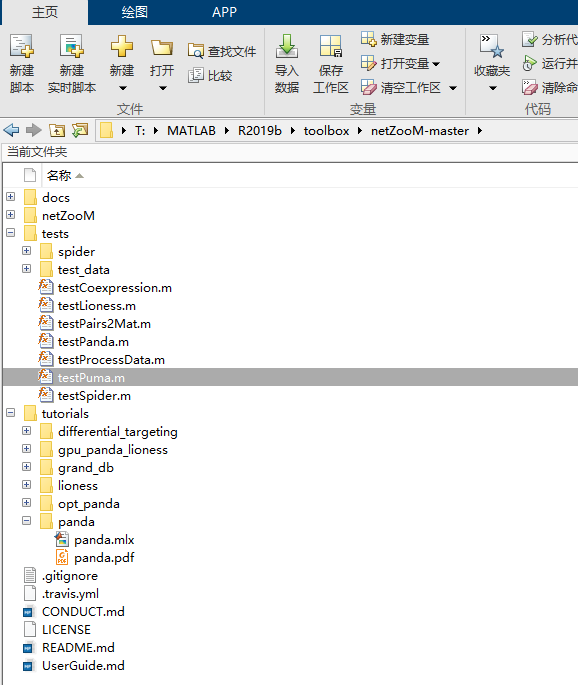
\includegraphics[width=0.46\textwidth]{pandamatlab2020032501.PNG}
\caption{netZooM (panda工具箱)}
\label{pandamatlab2020032501}
\end{figure}

%%%%%%%%%%%%%%%%%%%%%%%%%%%%%%%%%%%%%%%%%%
\section{记忆学习}

记忆学习(Rote learning)也叫死记硬背学习, 是一种最基本的学习过程, 它没有足够的能力独立完成智能学习, 但对学习系统来说都是十分重要的一个组成部分, 原因是任何学习系统都必须记住它们所获取的知识, 以便将来使用.

记忆学习的基本过程是: 执行元素每解决一个问题, 系统就记住这个问题和它的解, 当以后再遇到此类问题时, 系统就不必重新进行计算, 而可以直接找出原来的解去使用.

若把执行元素比作一个函数$f$, 由环境得到的输入模式记为$(x_1,x_2,\cdots ,x_n)$, 由该输入模式经$F$计算后得到的输出模式记为$(y_1,y_2,\cdots ,y_m)$, 则机械学习系统就是要把这一输入输出模式对:
\begin{align}
  [(x_1,x_2,\cdots ,x_n) , (y_1,y_2,\cdots ,y_m)]
\end{align}
保存在知识库中, 当以后再需要计算$f(x_1,x_2,\cdots ,x_n)$时, 就可以直接从存储器把$(y_1,y_2,\cdots ,y_m)$检索出来, 而不需要再重新进行计算.
%%%%%%%%%%%%%%%%%%%%%%%%%%%%%%%%%%%%%%%%%%
\begin{figure}[H]
\centering
\includegraphics[width=0.76\textwidth]{zhengxiangtuili2019112702.PNG}
\caption{机械式学习的学习模型}
\label{AI32fig2702}
\end{figure}
%%%%%%%%%%%%%%%%%%%%%%%%%%%%%%%%%%%%%%%%%%
%%%%%%%%%%%%%%%%%%%%%%%%%%%%%%%%%%%%%%%%%%
\section{机械式学习的学习模型}
%%%%%%%%%%%%%%%%%%%%%%%%%%%%%%%%%%%%%%%%%%
\subsection{归纳学习}
%%%%%%%%%%%%%%%%%%%%%%%%%%%
\begin{itemize}
\item 归纳学习是指以归纳推理为基础的学习, 其任务是要从关于某个概念的一系列已知的正例和反例中归纳出一个一般的概念描述.
\item 示例学习是归纳学习的一种特例. 它给学习者提供某一概念的一组正例和反例, 学习者归纳出一个总的概念描述, 并使这个描述适合于所有的正例, 排除所有的反例.
\item 决策树学习是一种以示例为基础的归纳学习方法, 也是目前最流行的归纳学习方法之一. 在现有的各种决策树学习算法中, 影响较大的是ID3算法. 本节主要讨论决策树的概念和决策树学习的ID3算法.
\end{itemize}
%%%%%%%%%%%%%%%%%%%%%%%%%%%%%%%%%%%%%%%%%%
\subsection{示例学习的类型}
%%%%%%%%%%%%%%%%%%%%%%%%%%%
\begin{itemize}
\item 按例子的来源分类

  \ding{172} 来源于教师的示例学习.

  \ding{173} 来源于学习者本身的示例学习.
\item 学习者明确知道自己的状态, 但完全不清楚所要获取的概念.

    \ding{171} 来源于学习者以外的外部环境的示例学习. 例子的产生是随机的.
\item 按例子的类型分类

    \ding{172} 仅利用正例的示例学习.

    这种学习方法会使推出的概念的外延扩大化.

    \ding{173} 利用正例和反例的示例学习.

    这是示例学习的一种典型方式, 它用正例用来产生概念, 用反例用来防止概念外延的扩大.
\end{itemize}
%%%%%%%%%%%%%%%%%%%%%%%%%%%%%%%%%%%%%%%%%%
\paragraph{示例学习的典型方式}
\begin{itemize}
\item 示例空间: 向系统提供的示教例子的集合. 研究问题: 例子质量, 搜索方法.
\item 解释过程: 是从搜索到的示例中抽象出一般性的知识的归纳过程. 解释方法: 常量转换为变量, 去掉条件, 增加选择, 曲线拟合等.
\item 规则空间: 是事务所具有的各种规律的集合. 研究问题: 对空间的要求, 搜索方法.
\item 验证过程: 是要从示例空间中选择新的示例, 对刚刚归纳出的规则做进一步的验证和修改.
\end{itemize}
%%%%%%%%%%%%%%%%%%%%%%%%%%%%%%%%%%%%%%%%%%%
%\begin{figure}[H]
%\centering
%\includegraphics[width=0.76\textwidth]{zhengxiangtuili2019112703.PNG}
%\caption{示例学习}
%\label{AI32fig2703}
%\end{figure}
%%%%%%%%%%%%%%%%%%%%%%%%%%%%%%%%%%%%%%%%%%%
%%%%%%%%%%%%%%%%%%%%%%%%%%%%%%
\begin{figure}[H]
\begin{center}
\begin{tikzpicture}[font={\sf \small}]
\def \smbwd{2cm}
\def \smbwe{4cm}
\thispagestyle{empty}
%定义流程图的具体形状
\node (slkj) at (0,0) [draw, process,minimum width=\smbwd, minimum height=0.5cm] {示例空间};      % 验证空间
\node (jsgc)[draw, process,align=center,right=2cm of slkj,yshift=-1.5cm] {解释过程};                 % 解释过程
\node (yzgc)[draw, process,right=2cm of slkj,minimum width=\smbwd, minimum height=0.5cm,yshift=1.5cm] {验证过程};                % 示例空间
\node (gzkj)[draw, process,align=center,right=6cm of slkj,yshift=0cm] {规则空间};                 % 规则空间
\draw[->,thick,blue] (slkj.south)|-(jsgc) node[left,yshift=0.25cm,xshift=-1cm] {};
\draw[->,thick,blue] (jsgc.east)-|(gzkj) node[left,yshift=0.25cm,xshift=-1cm] {};
\draw[->,thick] (gzkj.north)|-(yzgc.east) node[left,yshift=0.25cm,xshift=-1cm] {};
\draw[->,thick] (yzgc.west)-|(slkj.north) node[left,yshift=0.25cm,xshift=-1cm] {};
\end{tikzpicture}
\caption{示例学习}
\label{AI32fig2703}
\end{center}
\end{figure}
%%%%%%%%%%%%%%%%%%%%%%%%%%%%%%
%%%%%%%%%%%%%%%%%%%%%%%%%%%%%%%%%%%%%%%%%%
\section{示例学习的解释方法}
是指解释过程从具体示例形成一般性知识所采用的归纳推理方法. 最常用的解释方法有以下4种:
\begin{itemize}
\item (1) 把常量转换为变量: 把示例中的常量换成变量而得到一个一般性的规则.

\item(2) 去掉条件: 把示例中的某些无关的子条件舍去.

\item(3) 增加选择: 在析取条件中增加一个新的析取项. 常用的增加析取项的方法有前件析取法和内部析取法两种.

\item(4) 曲线拟合: 对数值问题的归纳可采用最小二乘法进行曲线拟合.
\end{itemize}
%%%%%%%%%%%%%%%%%%%%%%%%%%%%%%%%%%%%%%%%%%%%
\begin{example}
假设例子空间中有以下两个关于扑克牌中“同花”概念的示例:
花色($c_1$, 梅花) $\wedge$ 花色($c_2$, 梅花) $\wedge$ 花色($c_3$, 梅花) $\wedge$ 花色($c_4$, 梅花)$\wedge$ 花色($c_5$, 梅花) $\rightarrow$ 同花($c_1$, $c_2$, $c_3$, $c_4$, $c_5$).

花色($c_1$, 红桃) $\wedge$ 花色($c_2$, 红桃) $\wedge$ 花色($c_3$, 红桃) $\wedge$ 花色($c_4$, 红桃)$\wedge$ 花色($c_5$, 红桃) $\rightarrow$ 同花($c_1$, $c_2$, $c_3$, $c_4$, $c_5$).
\end{example}
其中, 示例1表示5张梅花牌是同花, 示例2表示5张红桃牌是同花.

解释过程:
%%%%%%%%%%%%%%%%%%%%%%%%%%%%%%%%%%%%%%%%%%%%
\begin{itemize}
\item (1) 把常量化为变量
\begin{example}
对这两个示例, 只要把“梅花”和“红桃”用变量$x$代换, 就可得到如下一般性的规则:

    规则1: 花色($c_1$, x) $\wedge$ 花色($c_2$, x) $\wedge$ 花色($c_3$, x) $\wedge$ 花色($c_4$, x)$\wedge$ 花色($c_5$, x)$\rightarrow$ 同花($c_1$, $c_2$, $c_3$, $c_4$, $c_5$).
\end{example}

\item (2)去掉条件: 把示例中的某些无关的子条件舍去.

%%%%%%%%%%%%%%%%%%%%%%%%%%%%%%%%%%%%%%%%%%%%
\begin{example}
  花色($c_1$, 红桃)$\wedge$点数($c_1$, 2)
            $\wedge$花色($c_2$, 红桃)$\wedge$点数($c_2$, 3)
            $\wedge$花色($c_3$, 红桃)$\wedge$点数($c_3$, 4)
            $\wedge$花色($c_4$, 红桃)$\wedge$点数($c_4$, 5)
            $\wedge$花色($c_5$, 红桃)$\wedge$点数($c_5$, 6)
          $\rightarrow$ 同花($c_1$, $c_2$, $c_3$, $c_4$, $c_5$)
\end{example}

为了学习同花的概念, 除了需要把常量变为变量外, 还需要把与花色无关的“点数”子条件舍去. 这样也可得到上述规则1:

$\bullet$ 规则1: 花色($c_1$, x) $\wedge$ 花色($c_2$, x) $\wedge$ 花色($c_3$, x) $\wedge$ 花色($c_4$, x)$\wedge$ 花色($c_5$, x)$\rightarrow$ 同花($c_1$, $c_2$, $c_3$, $c_4$, $c_5$).

\item (3)增加选择: 在析取条件中增加一个新的析取项. 包括前件析取法和内部析取法.

\textbf{前件析取法}: 是通过对示例的前件的析取来形成知识的.

%%%%%%%%%%%%%%%%%%%%%%%%%%%%%
\begin{example}示例的前件有4个:
%%%%%%%%%%%%%%%%%%%%%%%%%%%%%%%%%%%%%%%%%%%%
\begin{itemize}
\item 点数($c_1$, J)$\rightarrow$脸($c_1$)
\item 点数($c_1$, Q)$\rightarrow$脸($c_1$)
\item 点数($c_1$, K)$\rightarrow$脸($c_1$)
\end{itemize}

将各示例的前件进行析取, 就可得到所要求的规则:

 $\bullet$ 规则2: 点数($c_1$, J)∨点数($c_1$, Q)∨点数($c_1$, K)$\rightarrow$脸($c_1$)
\end{example}

\textbf{内部析取法}: 是在示例的表示中使用集合与集合的成员关系来形成知识的.

%%%%%%%%%%%%%%%%%%%%%%%%%%%%%
\begin{example}
有如下关于“脸牌”的示例:
%%%%%%%%%%%%%%%%%%%%%%%%%%%%%%%%%%%%%%%%%%%%
\begin{itemize}
\item 点数$c_1\in {J}\rightarrow$脸($c_1$)
\item 点数$c_1\in {Q}\rightarrow$脸($c_1$)
\item 点数$c_1\in {K}\rightarrow$脸($c_1$)
\end{itemize}

用内部析取法, 可得到如下规则:

$\bullet$ 规则3: 点数$(c_1)\in {J, Q, K}\rightarrow$脸($c_1$)
\end{example}
\item (4)曲线拟合: 对数值问题的归纳可采用曲线拟合法.
\end{itemize}
假设示例空间中的每个示例$(x, y, z)$都是输入$x, y$与输出$z$之间关系的三元组.
\begin{example}
有下3个示例:
%%%%%%%%%%%%%%%%%%%%%%%%%%%%%%%%%%%%%%%%%%%%
\begin{itemize}
\item (0, 2, 7)
\item (6, -1, 10)
\item (-1, -5, -16)
\end{itemize}

用最小二乘法进行曲线拟合, 可得$x, y, z$之间关系的规则如下:

$\bullet$ 规则4: $z=2x+3y+1$.
\end{example}
%%%%%%-------------------------------------------------
\begin{remark}
在上述前三种方法中, 方法(1)是把常量转换为变量;方法(2)是去掉合取项(约束条件);方法(3)是增加析取项. 它们都是要扩大条件的适用范围. 从归纳速度上看, 方法(1)的归纳速度快, 但容易出错;方法(2)归纳速度慢, 但不容易出错. 因此, 在使用方法(1)时应特别小心.

%%%%%%%%%%%%%%%%%%%%%%%%%%%%%
\begin{example}
对示例4、示例5及示例6, 若使用方法(1) ,则会归纳出如下的错误规则:

规则5: (错误)点数($c_1$, $x$)$\rightarrow$脸($c_1$),

它说明, 归纳过程是很容易出错的.
\end{example}
\end{remark}

决策树是一种由节点和边构成的用来描述分类过程的层次数据结构. 该树的根接点表示分类的开始, 叶节点表示一个实例的结束, 中间节点表示相应实例中的某一属性, 而边则代表某一属性可能的属性值.
在决策树中, 从根节点到叶节点的每一条路径都代表一个具体的实例, 并且同一路径上的所有属性之间为合取关系, 不同路径(即一个属性的不同属性值)之间为析取关系.
决策树的分类过程就是从这棵树的根接点开始, 按照给定的事例的属性值去测试对应的树枝, 并依次下移, 直至到达某个叶节点为止.

图\ref{AI32fig2704}是一个非常简单的用来描述对鸟类进行分类的决策树.
在该图中: 根节点包含各种鸟类, 叶节点是所能识别的各种鸟的名称; 中间节点是鸟的一些属性, 边是鸟的某一属性的属性值; 从根节点到叶节点的每一条路径都描述了一种鸟, 它包括该种鸟的一些属性及相应的属性值.
%%%%%%%%%%%%%%%%%%%%%%%%%%%%%%%%%%%%%%%%%%
\begin{figure}[H]
\centering
\includegraphics[width=0.76\textwidth]{zhengxiangtuili2019112704.PNG}
\caption{对鸟类进行分类的决策树}
\label{AI32fig2704}
\end{figure}
%%%%%%%%%%%%%%%%%%%%%%%%%%%%%%%%%%%%%%%%%%
 决策树还可以表示成规则的形式. 上图\ref{AI32fig2704}的决策树可表示为如下规则集:
\begin{Verbatim}
    IF  鸟类会飞       AND  是家养的          THEN  该鸟类是和平鸽
    IF  鸟类会飞       AND  不是家养的      THEN  该鸟类是信天翁
    IF  鸟类不会飞   AND  会游泳              THEN  该鸟类是企鹅
    IF  鸟类不会飞   AND  不会游泳         THEN  该鸟类是鸵鸟
\end{Verbatim}

决策树学习过程实际上是一个构造决策树的过程. 当学习完成后, 就可以利用这棵决策树对未知事物进行分类.
%%%%%%%%%%%%%%%%%%%%%%%%%%%%%%%%%%%%%%%%%%
\subsection{ID3算法}
D3算法是昆兰(J.R.Quinlan)于1979年提出的一种以信息熵(entropy)的下降速度作为属性选择标准的一种学习算法. 其输入是一个用来描述各种已知类别的例子集, 学习结果是一棵用于进行分类的决策树.

%%%%%%%%%%%%%%%%%%%%%%%%%%%%%%%%%%%%%%%%%%
\paragraph{ID3算法的数学基础}
先引入信息熵和条件熵的数学概念
%%%%%%%%%%%%%%%%%%%%%%%%%%%%%%%%%%%%%%%%%%
\subparagraph{信息熵}
信息熵是对信息源整体不确定性的度量. 假设$X$为信源, $x_i$为$X$所发出的单个信息, $P(x_i)$为X发出$x_i$的概率, 则信息熵可定义为:
\begin{align}
  \begin{aligned}
  H(X) &=-P\left(x_{1}\right) \log P\left(x_{1}\right)-P\left(x_{2}\right) \log P\left(x_{2}\right)-\cdots-P\left(x_{r}\right) \log P\left(x_{r}\right) \\
                       &=-\sum_{i=1}^{k} P\left(x_{i}\right) \log P\left(x_{i}\right)
  \end{aligned}
\end{align}
其中, $k$为信源$X$发出的所有可能的信息类型, 对数可以是以各种数为底的对数, 在ID3算法中, 我们取以2为底的对数.
%%%%%%%%%%%%%%%%%%%%%%%%%%%%%%%%
\begin{remark}
 信息熵反应的是信源每发出一个信息所提供的平均信息量.
\end{remark}
%%%%%%%%%%%%%%%%%%%%%%%%%%%%%%%%%%%%%%%%%%
\subparagraph{条件熵}
条件熵是收信者在收到信息后对信息源不确定性的度量. 若假设信源为$X$, 收信者收到的信息为$Y$,  $P(x_i/y_j)$为当Y为$y_j$时$X$为$x_i$的条件概率, 则条件熵可定义为:
\begin{align}
  H(X | Y)=-\sum_{i}^{k} \sum_{j}^{k} P\left(x_{i} | y_{j}\right) \log P\left(x_{i} | y_{j}\right)
\end{align}
它表示收信者收到$Y$后对$X$不确定性的估计.

%%%%%%%%%%%%%%%%%%%%%%%%%%%%%%%%%%%%%%%%%%
\paragraph{ID3算法及举例}
ID3算法的学习过程:
\begin{itemize}
\item 首先以整个例子集作为决策树的根节点$S$, 并计算$S$关于每个属性的期望熵(即条件熵);
\item 然后选择能使$S$的期望熵为最小的一个属性对根节点进行分裂, 得到根节点的一层子节点;
\item 接着再用同样的方法对这些子节点进行分裂, 直至所有叶节点的熵值都下降为0为止.
\end{itemize}
这时, 就可得到一棵与训练例子集对应的熵为0的决策树, 即ID3算法学习过程所得到的最终决策树. 该树中每一条从根节点到叶节点的路径, 都代表了一个分类过程, 即决策过程.

%%%%%%%%%%%%%%%%%%%%%%%%%%%%%%%%%%%
\begin{example}
用ID3算法完成下述学生选课

假设将决策$y$分为以下3类:
\begin{Verbatim}
    $y_1$: 必修AI
    $y_2$: 选修AI
    $y_3$: 不修AI
\end{Verbatim}

做出这些决策的依据有以下3个属性:
\begin{Verbatim}
    $x_1$: 学历层次 $x_1=1$ 研究生, $x_1=2$ 本科
    $x_2$: 专业类别 $x_2=1$ 电信类, $x_2=2$ 机电类
    $x_3$: 学习基础 $x_3=1$ 修过AI, $x_3=2$ 未修AI
\end{Verbatim}
\end{example}

表\ref{AItable20122435}给出了一个关于选课决策的训练例子集$S$. 在该表中, 训练例子集$S$的大小为. ID3算法是依据这些训练例子, 以$S$为根节点, 按照信息熵下降最大的原则来构造决策树的.
%%%%%%%%%%%%%%%%%%%%%%%%%%%%%%%
\begin{table} [!tb]
\caption{关于选课决策的训练例子集}
\vspace{-0.2cm}
\begin{center}
\begin{tabular} {lccccc}
\hline
序号&	属性值	&&&决策方案\\
\hline
$y_i$&$x_1$&$x_2$&$x_3$\\
1	&1	&1	&1&	$y_3$\\
2	&1&	1&	2&	$y_1$\\
3	&1&2&1&$y_3$\\
4&1&2&2&$y_2$\\
5&2&1&1&$y_3$\\
6&2&1&2&$y_2$\\
7&2&2&1&$y_3$\\
8&2&2&2&$y_3$\\
\hline
\end{tabular}
\end{center}
\label{AItable20122435}
\end{table}

解:  首先对根节点, 其信息熵为:
\begin{align}
  H(S)=-\sum_{i=1}^{3} P\left(y_{i}\right) \log_ {2} P\left(y_{i}\right)
\end{align}
其中, 为可选的决策方案数, 且有
\begin{align}
  P(y_1)=\frac 1 8, P(y_2)=\frac 2 8, P(y_3)=\frac 5 8
\end{align}
即有:
\begin{align}
    H(S)= -\left(\frac 1 8\right)\log_2 \left(\frac 1 8\right)- \left(\frac 2 8\right)\log_ 2\left(\frac 2 8 \right)- \left(\frac 5 8\right)\log_ 2\left(\frac 5 8\right) =1.2988.
\end{align}

按照ID3算法, 需要选择一个能使$S$的期望熵为最小的一个属性对根节点进行扩展, 因此我们需要先计算$S$关于每个属性的条件熵:
\begin{align}
  H\left(S / x_{i}\right)=\sum_{t} \frac{\left|S_{t}\right|}{|S|} H\left(S_{i}\right)
\end{align}
其中, $t$为属性$x_i$的属性值, $S_t$为$x_i=t$时的例子集, $|S|$和$|S_i|$分别是例子集$S$和$S_i$的大小.

下面先计算$S$关于属性$x_1$的条件熵:
\begin{align}
  H\left(S / x_{i}\right)=\sum_{t} \frac{\left|S_{t}\right|}{|S|} H\left(S_{i}\right)
\end{align}
在表7-1中, $x_1$的属性值可以为1或2. 当$x_1=1$时, $t=1$时, 有:
\begin{align}
  S_1=\{1, 2, 3, 4\}
\end{align}
当$x_1=2$时, $t=2$时, 有:
\begin{align}
  S_2=\{5, 6, 7, 8\}
\end{align}
其中, $S_1$和$S_2$中的数字均为例子集S中的各个例子的序号, 且有$|S|=8,|S_1|=|S_2|=4$.

由$S_1$可知:
\begin{align}
  P_{s_1}(y_1)=1/4,     P_{s_1}(y_2)=1/4,     P_{s_1}(y_3)=2/4
\end{align}
则有:
\begin{align}
H(S_1)&= - P_{s1}(y_1)\log_2 P_{s1}(y_1) - P_{s_1}(y_2)\log_2 P_{s1}(y_2 )- P_{s_1}(y_3)\log_2 P_{s_1}(y_3 )\\
     &= -(1/4)\log_2(1/4)- (1/4)\log_2(1/4)- (2/4)\log_2(2/4) =1.5
\end{align}

再由$S_2$可知:
\begin{align}
  P_{s_2}(y_1)=\frac 0 4, P_{s_2}(y_2)=\frac 1 4, P_{s_2}(y_3)=\frac 3 4
\end{align}
则有:
\begin{align}
    H(S_2)&=– P_{s_2}(y_2)log2 P_{s_2}(y_2 )- P_{s_2}(y_3)log_2\\
    P_{s_2}(y_3)&=-\frac 1 4\log_2\left(\frac 1 4\right)- \left(\frac 3 4\right)\log_2\left(\frac 3 4\right) =0.8113.
\end{align}
将$H(S_1)$和$H(S_2)$代入条件熵公式, 有:
\begin{align}
    H(S/x_1)=(|S_1|/|S|)H(S_1)+ (|S_2|/|S|)H(S_2)=\left(\frac 4 8\right)\times 1.5+\left(\frac 4 8\right)\times 0.8113 =1.1557.
\end{align}
同样道理, 可以求得:
\begin{align}
  &H(S/x_2)=1.1557\\
  &H(S/x_3)=0.75
\end{align}
可见, 应该选择属性$x_3$对根节点进行扩展. 用$x_3$对$S$扩展后所得到的得到部分决策树如图\ref{bufenjueceshu2019112901}所示.
%%%%%%%%%%%%%%%%%%%%%%%%%%%%%%%%%%%%%%%%%%%
%\begin{figure}[H]
%\centering
%\includegraphics[width=0.6\textwidth]{bufenjueceshu20191129}
%\caption{部分决策树}
%\label{bufenjueceshu2019112901}
%\end{figure}
%%%%%%%%%%%%%%%%%%%%%%%%%%%%%%%%%%%%%%%%%%%
%%%%%%%%%%%%%%%%%%%%%%%%%%%%%%
\begin{figure}[H]
\begin{center}
\begin{tikzpicture}[font={\sf \small}]
\def \smbwd{2cm}
\def \smbwe{4cm}
\thispagestyle{empty}
%定义流程图的具体形状
\node (x31y3)[draw, process,align=center,right=2cm of slkj] {$x_3=1,y_3$};
\node (S) at (0,0) [draw, process,right=2cm of x31y3,minimum width=\smbwd, minimum height=0.5cm,yshift=2.05cm] {$S$};
\node (x32x1x2)[draw, process,right=5cm of x31y3,minimum width=\smbwd, minimum height=0.5cm] {$x_3=2,x_1,x_2$};
\draw[thick,blue] (x31y3.east)--(S.south) node[left,yshift=-0.55cm,xshift=-1.65cm,rotate=29] {$x_3=1$};
\draw[thick,blue] (x32x1x2.north)--(S.south) node[left,yshift=-0.75cm,xshift=2.65cm,rotate=-30] {$x_3=2$};
\end{tikzpicture}
\caption{部分决策树}
\label{bufenjueceshu2019112901}
\end{center}
\end{figure}
%%%%%%%%%%%%%%%%%%%%%%%%%%%%%%
在该树中, 节点“$x_3=1, y_3$”表示当$x_3$的属性值为1时, 得到决策方案$y_3$. 由于$y_3$已是具体的决策方案, 故该节点的信息熵为0, 已经为叶节点.

节点“$x_3=2, x_1,x_2$”的含义是“当$x_3$的属性值为2时, 还需要考虑属性$x_1,x_2$”, 它是一个中间节点, 还需要继续扩展.

至于节点“$x_3=2, x_1,x_2$”, 其扩展方法与上面的过程类似. 通过计算可知, 该节点对属性$x_1$和$x_2$, 其条件熵均为1. 由于它对属性$x_1$和$x_2$的条件熵相同, 因此可以先选择$x_1$, 也可以先选择$x_2$, 本例是先选择$x_2$.

依此进行下去, 可得到如图\ref{bufenjueceshu2019112902}所示的最终的决策树. 在该决策树中, 各节点的含义与图\ref{bufenjueceshu2019112901}类似.
%%%%%%%%%%%%%%%%%%%%%%%%%%%%%%%%%%%%%%%%%%
\begin{figure}[H]
\centering
\includegraphics[width=0.6\textwidth]{bufenjueceshu20191130.png}
\caption{最终决策树}
\label{bufenjueceshu2019112902}
\end{figure}
%%%%%%%%%%%%%%%%%%%%%%%%%%%%%%%%%%%%%%%%%%
%%%%%%%%%%%%%%%%%%%%%%%%%%%%%%%%%%%%%%%%%%
\subsection{解释学习的空间描述}
解释学习涉及三个不同的空间: 例子空间, 概念空间和概念描述空间. 三个空间及它们之间的关系如图\ref{AI32fig2705}所示.

概念描述空间是所有概念描述的集合, 其中的概念描述可分为两大类, 一类是可操作的, 另一类是不可操作的. 所谓可操作是指一个概念描述能有效的用于识别相应概念的例子. 否则是不可操作的. 解释学习的任务就是要把不可操作的概念描述转化为可操作的概念描述.

概念空间是学习过程能够描述的所有概念的集合. 例子空间是用于问题求解的例子集合
%%%%%%%%%%%%%%%%%%%%%%%%%%%%%%%%%%%%%%%%%%
\begin{figure}[H]
\centering
\includegraphics[width=0.6\textwidth]{zhengxiangtuili2019112705.PNG}
\caption{解释学习的三个空间}
\label{AI32fig2705}
\end{figure}
%%%%%%%%%%%%%%%%%%%%%%%%%%%%%%%%%%%%%%%%%%
%%%%%%%%%%%%%%%%%%%%%%%%%%%%%%%%%%%%%%%%%%
\subsection{解释学习的模型}
模型组成说明:

1) EXL 为学习系统

2) KB 为领域知识库, 它是不同概念描述之间进行转换所使用的规则集合;

3) PS 为执行系统;

4) D1 是输入的概念描述, 一般为不可操作的;

5) D2 是学习结束时输出的概念描述, 它是可操作的.

执行过程: 先由EXL接受输入的概念描述D1, 然后再根据KB中的知识对D1进行不同描述的转换, 并由PS对每个转换结果进行测试, 直到被PS所接受, 即为可操作的概念描述D2为止;最后输出D2.

%%%%%%%%%%%%%%%%%%%%%%%%%%%%%%%%%%%%%%%%%%
\begin{figure}[H]
\centering
\includegraphics[width=0.76\textwidth]{zhengxiangtuili2019112706.PNG}
\caption{解释学习模型}
\label{AI32fig2706}
\end{figure}
%%%%%%%%%%%%%%%%%%%%%%%%%%%%%%%%%%%%%%%%%%

%%%%%%%%%%%%%%%%%%%%%%%%%%%%%%%%%%%%%%%%%%
\subsection{解释学习的基本原理}
本节主要讨论米切尔等人提出的解释泛化学习方法.
%%%%%%%%%%%%%%%%%%%%%%%%%%%%%%%%%%%%%%%%%%
\paragraph{解释泛化学习方法-1}
其基本思想: 先对某一情况建立一个解释结构, 然后在对此解释结构进行概括, 获取一般性控制知识.

其一般性描述为: 已知:
\begin{itemize}
\item 目标概念GC(Goal Concept);
      \begin{itemize}
          \item 训练实例TE(Training Example);
          \item 领域理论DT(Domain Theory);
           \item 操作性标准OC(Operationality Criterion).
       \end{itemize}
\item \textbf{求出}: 满足OC的关于GC的充分概念描述, 其中: 目标概念GC 是要学习概念的描述.
\end{itemize}

\begin{itemize}
\item 训练实例TE为学习系统提供的一个实例;
\item 领域理论DT是相关领域的事实和规则, 即为背景知识;
\item 操作性标准OC用于指导学习系统对用来描述目标的概念进行舍取等的控制性知识.
\end{itemize}
%%%%%%%%%%%%%%%%%%%%%%%%%%%%%%%%%%%%%%%%%%
\paragraph{解释泛化学习方法-2}
本节主要讨论米切尔等人提出的解释泛化学习方法.
解释泛化学习的基本思想: 先对某一情况建立一个解释结构, 然后在对此解释结构进行概括, 获取一般性控制知识.

其一般性描述为: 已知:
\begin{itemize}
\item 目标概念GC(Goal Concept);
   \begin{itemize}
         \item 训练实例TE(Training Example);
         \item 领域理论DT(Domain Theory);
         \item 操作性标准OC(Operationality Criterion).
   \end{itemize}
\item \textbf{求出}: 满足$OC$的关于$GC$的充分概念描述.
\end{itemize}
其中: 目标概念$GC$是要学习概念的描述.

\begin{itemize}
\item 训练实例TE是为学习系统提供的一个实例;
\item 领域理论DT 是相关领域的事实和规则, 即为背景知识;
\item 操作性标准OC 用于指导学习系统对用来描述目标的概念进行舍取等的控制性知识.
\end{itemize}

其任务是要证明提供给系统的训练实例为什么是目标概念的一个实例. 为此, 系统应从目标开始反向推理, 根据知识库中已有的事实和规则分解目标, 直到求解结束. 一旦得到解, 便完成了该问题的证明, 同时也获得了一个解释结构.

%%%%%%%%%%%%%%%%%%%%%%%%%%%%%%%%%
\begin{example}
假设要学习的目标是“一个物体$x$可以安全地放置在另一个物体$y$的上面”. 即目标概念:
\begin{center}
  Safe-to-Stack ($x, y$)
\end{center}

训练实例(是一些描述物体$\textup{obj}_1$与$\textup{obj}_2$的事实):
\begin{Verbatim}
       On(obj1 ,obj2)         物体1在物体2的上面
       Isa(obj1 , book)       物体1是书
       Isa(obj2 , table)      物体2是桌子
       Volume(obj1 , 1)       物体1的体积是1
       Density(obj1 , 0.1)    物体1的密度是0.1
\end{Verbatim}

领域知识   是把一个物体安全地放置在另一个物体上面的准则:
\begin{center}
  $\neg $Fragile(y)$\rightarrow$Safe-to-stack($x, y$)
\end{center}
\end{example}

如果$y$不是易碎的, 则$x$可以安全地放到$y$的上面
\begin{center}
  Lighter(x, y)$\rightarrow$Safe-to-stack($x, y$)
\end{center}

如果$x$比$y$轻, 则$x$可以安全地放到$y$的上面
\begin{center}
  Volume(p, v)$\wedge$Density(p, d)$\wedge$Product ($v, d, w$)$\rightarrow$Weight($p, w$)
\end{center}

如果$p$的体积是$v$、密度是$d$、$v$乘以$d$的积是$w$, 则$p$的重量是$w$
\begin{center}
  Is-a(p, table)$\rightarrow$Weight(p, 5)
\end{center}

如果$p$是桌子, 则$p$的重量是5
\begin{center}
  Weight($p_1, w_1$)$\wedge$Weight($p_2,w_2$)$\wedge$Smaller($w_1, w_2$)$\rightarrow$Lighter($p_1, p_2$)
\end{center}

如果$p_1$的重量是$w_1, p_2$的重量是$w_2,w_1$比$w_2$小,  则$p_1$比$p_2$轻.

其证明过程是一个由目标引导的逆向推理, 最终得到的解释树就是该例的解释结构(如图\ref{AI32fig2707}).
%%%%%%%%%%%%%%%%%%%%%%%%%%%%%%%%%%%%%%%%%%
\begin{figure}[H]
\centering
\includegraphics[width=0.76\textwidth]{zhengxiangtuili2019112707.PNG}
\caption{逆向推理的解释树}
\label{AI32fig2707}
\end{figure}
%%%%%%%%%%%%%%%%%%%%%%%%%%%%%%%%%%%%%%%%%%

这一步的主要任务是对上一步得到的解释结构进行概括化处理, 从而得到关于目标概念的一般性知识.
     进行概括化处理的常用方法是把常量转换为变量, 即把某些具体数据换成变量, 并略去某些不重要的信息, 只保留求解所必须的那些关键信息即可.
     对上图的解释结构进行概括化处理以后所得到的概括化解释结构如下:
%%%%%%%%%%%%%%%%%%%%%%%%%%%%%%%%%%%%%%%%%%
\begin{figure}[H]
\centering
\includegraphics[width=0.76\textwidth]{zhengxiangtuili2019112708.PNG}
\caption{概括化解释结构}
\label{AI32fig2708}
\end{figure}
%%%%%%%%%%%%%%%%%%%%%%%%%%%%%%%%%%%%%%%%%%
 将该解释结构中所有的叶节点的合取作为前件, 顶点的目标概念做为后件, 略去解释结构的中间部件, 就可得到概括化的一般性知识:
\begin{align}
  \textup{Volume}(O_1,v_1)&\wedge \textup{Density}(O_1,d_1)\wedge \textup{Product}(v_1,d_1,w_1)\notag\\
                          &\wedge \textup{Is}-a(O_2,\textup{table})\wedge\textup{Smaller}(w_1,5)\rightarrow \textup{Safe-to-stack}(O_1,O_2)
\end{align}
%%%%%%%%%%%%%%%%%%%%%%%%%%%%%%%%%%%%%%%%%%
\subsection{浅层神经学习的心理学基础}

神经生理学研究表明, 人脑的神经元既是学习的基本单位, 同是也是记忆的基本单位. 目前, 关于人脑学习和记忆机制的研究有两大学派:
\begin{itemize}
\item 化学学派: 认为人脑经学习所获得的信息是记录在某些生物大分子之上的. 例如, 蛋白质、核糖核酸、神经递质, 就像遗传信息是记录在DNA(脱氧核糖核酸)上一样.
\item 突触修正学派: 认为人脑学习所获得的信息是分布在神经元之间的突触连接上的.
\end{itemize}
按照突触修正学派的观点, 人脑的学习和记忆过程实际上是一个在训练中完成的突触连接权值的修正和稳定过程. 其中, 学习表现为突触连接权值的修正, 记忆则表现为突触连接权值的稳定.

突触修正假说已成为人工神经网络学习和记忆机制研究的心理学基础, 与此对应的权值修正学派也一直是人工神经网络研究的主流学派.
突触修正学派认为, 人工神经网络的学习过程就是一个不断调整网络连接权值的过程.

所谓学习规则可简单地理解为学习过程中联结权值的调整规则. 按照学习规则, 神经学习可分为\uwave{Hebb学习、纠错学习、竞争学习及随机学习}等.

    (1) \textbf{Hebb学习} 基本思想: 如果神经网络中某一神经元同另一直接与它连接的神经元同时处于兴奋状态, 那么这两个神经元之间的连接强度将得到加强, 反之应该减弱.

Hebb学习对连接权值的调整可表示为:
\begin{align}
  w_{i j}(t+1)=w_{i j}(t)+\eta\left[x_{i}(t) x_{j}(t)\right],
\end{align}
其中, $w_{ij}(t+1)$表示对时刻$t$的权值修正一次后所得到的新的权值;$\eta$是一正常量, 也称为学习因子, 它取决于每次权值的修正量;
$x_i(t)$、$x_j(t)$分别表示$t$时刻第$i$个和第$j$个神经元的状态.
Hebb学习规则在人工神经网络学习中的影响比较大, 但不符合生物机理. 例如习惯化.

  (2) \textbf{纠错学习} 是一种有导师的学习过程, 其基本思想:

利用神经网络的期望输出与实际输出之间的偏差作为连接权值调整的参考, 并最终减少这种偏差.

最基本的误差修正规则为: 连接权值的变化与神经元希望输出和实际输出之差成正比. 其联结权值的计算公式为:
\begin{align}
  w_{i j}(t+1)=w_{i j}(t)+\eta\left[d_{j}(t)-y_{j}(t)\right] x_{i}(t),
\end{align}
其中,  $w_{ij}(t)$表示时刻$t$的权值; $w_{ij}(t+1)$表示对时刻$t$的权值修正一次后所得到的新的权值;$\eta$是一正常量, 也称为学习因子;$y_j(t)$为神经元$j$的实际输出; $d_j(t)$为神经元$j$的希望输出;$d_j(t)-y_j(t)$表示神经元$j$的输出误差;$x_i(t)$为第$i$个神经元的输入.

(3) \textbf{竞争学习} 基本思想: 网络中某一组神经元相互竞争对外界刺激模式响应的权力, 在竞争中获胜的神经元, 其连接权会向着对这一刺激模式竞争更为有利的方向发展.

(4) \textbf{随机学习} 基本思想: 结合随机过程、概率和能量(函数)等概念来调整网络的变量, 从而使网络的目标函数达到最大(或最小). 他不仅可以接受能量函数减少(性能得到改善)的变化, 而且还可以以某种概率分布接受使能量函数增大(性能变差)的变化.
%%%%%%%%%%%%%%%%%%%%%%%%%%%%%%%%%%%%%%%%%%
\subsection{感知器学习}

单层感知器学习实际上是一种基于纠错学习规则, 采用迭代的思想对连接权值和阈值进行不断调整, 直到满足结束条件为止的学习算法.

假设$X(k)$和$W(k)$分别表示学习算法在第$k$次迭代时输入向量和权值向量, 为方便, 把阈值$\theta$作为权值向量$W(k)$中的第一个分量, 对应地把“-1”固定地作为输入向量$X(k)$中的第一个分量. 即$W(k)$和$X(k)$可分别表示如下:
\begin{align}
X(k)&=[-1, x_1(k), x_2(k),\cdots, x_n(k)]\\
W(k)&=[\theta(k),w_1(k), w_2(k),\cdots,w_n(k)];
\end{align}
即$x_0(k)=-1, w_0(k)=θ(k)$.

单层感知器学习是一种有导师学习, 它需要给出输入样本的期望输出.

假设一个样本空间可以被划分为$A, B$两类. 其功能函数的定义为: 对属于$A$类输入样本, 其功能函数的输出为+1, 否则其输出为-1. 对应地也可将期望输出定义为: 当输入样本属于$A$类时, 其期望输出为+1, 否则为-1.

单层感知器学习算法描述:

     (1) 设$t=0$, 初始化连接权和阈值. 即给$w_i(0)\,(i=1, 2, \cdots,n)$及$\theta(0)$分别赋予一个较小的非零随机数, 作为初值. 其中, $w_i(0)$是第0次迭代时输入向量中第$i$个输入的连接权值;$\theta(0)$是第0次迭代时输出节点的阈值;

     (2) 提供新的样本输入$x_i(t)\,(i=1, 2,\cdots, n)$和期望输出$d(t)$;

     (3) 计算网络的实际输出:
        \begin{align}
          y(t)=f\left(\sum_{i=1}^{n} w_{i}(t) x_{i}(t)-\theta(t)\right) \quad i=1,2, \ldots, n
        \end{align}

     (4) 若$y(t)=1$, 不需要调整连接权值, 转(6). 否则, 转(5) 调整连接权值
        \begin{align}
          w_{i}(t+1)=w_{i}(t)+\eta[d(t)-y(t)] x_{i}(t) \quad i=1,2, \ldots, n
        \end{align}
        其中, $\eta$是一个增益因子, 用于控制修改速度, 其值如果太大, 会影响$w_i(t)$的收敛性;如果太小, 又会使$w_i(t)$的收敛速度太慢;

     (6) 判断是否满足结束条件, 若满足, 算法结束;否则, 将$t$值加1, 转(2)重新执行. 这里的结束条件一般是指$w_i(t)$对一切样本均稳定不变.

    如果输入的两类样本是线性可分的, 则该算法就一定会收敛. 否则, 该算法将不收敛.
%%%%%%%%%%%%%%%%%%%%%%%%%%%%%%%%%%%%
\begin{example}
  用单层感知器实现逻辑“与”运算.
\end{example}
\begin{result}
根据“与”运算的逻辑关系, 可将问题转换为:

输入向量: $X_1=[0, 0, 1, 1],X_2=[0, 1, 0, 1]$,

输出向量: $Y=[0, 0, 0, 1]$.

为减少算法的迭代次数, 设初始连接权值和阈值取值如下:
\begin{align}
  w_1(0)=0.5,   w_2(0)=0.7,   \theta(0)=0.6,
\end{align}
并取增益因子$\eta=0.4$.
\end{result}

\textbf{算法的学习过程如下}:

设两个输入为$x_1(0)=0$和$x_2(0)=0$, 其期望输出为$d(0)=0$, 实际输出为:
\begin{align}
y(0)&=f(w_1(0)x_1(0)+ w_2(0)x_2(0)-\theta(0))\notag\\
    &=f(0.5*0+0.7*0-0.6)=f(-0.6)=0.
\end{align}
实际输出与期望输出相同, 不需要调节权值.

再取下一组输入: $x_1(0)=0$和$x_2(0)=1$,  期望输出$d(0)=0$, 实际输出:
\begin{align}
y(0)&=f(w_1(0) x_1(0)+ w_2(0) x_2(0)-\theta(0))\notag\\
    &=f(0.5*0+0.7*1-0.6)=f(0.1)=1.
\end{align}

实际输出与期望输出不同, 需要调节权值, 其调整如下:
\begin{align}
\theta(1)&=\theta(0)+\eta (d(0)- y(0))*(-1)=0.6+0.4*(0-1)*(-1)=1\\
w_1(1)&=w_1(0)+\eta (d(0)- y(0))x_1(0)=0.5+0.4*(0-1)*0=0.5\\
w_2(1)&=w_2(0)+\eta (d(0)- y(0))x_2(0)=0.7+0.4*(0-1)*1=0.3.
\end{align}

取下一组输入: $x_1(1)=1$和$x_2(1)=0$, 其期望输出为$d(1)=0$, 实际输出为:
\begin{align}
y(1)&=f(w_1(1) x_1(1)+ w_2(1) x_2(1)-\theta(1))\notag\\
    &=f(0.5*1+0.3*0-1)=f(-0.51)=0.
\end{align}
实际输出与期望输出相同, 不需要调节权值.

再取下一组输入: $x_1(1)=1$和$x_2(1)=1$, 其期望输出为$d(1)=1$, 实际输出为:
\begin{align}
  y(1)&=f(w_1(1) x1(1)+ w2(1) x_2(1)-\theta(1))\notag\\
      &=f(0.5*1+0.3*1-1)=f(-0.2)=0.
\end{align}
实际输出与期望输出不同, 需要调节权值, 其调整如下:
\begin{align}
\theta(2)&=\theta(1)+\eta (d(1)- y(1))*(-1)=1+0.4*(1-0)*(-1)=0.6\\
w_1(2)&=w_1(1)+\eta (d(1)- y(1))x_1(1)=0.5+0.4*(1-0)*1=0.9\\
w_2(2)&=w_2(1)+\eta (d(1)- y(1))x_2(1)=0.3+0.4*(1-0)*1=0.7.
\end{align}
取下一组输入: $x_1(2)=0$和$x_2(2)=0$, 其期望输出为$d(2)=0$, 实际输出为:
\begin{align}
  y(2)=f(0.9*0+0.7*0-0.6)=f(-0.6)=0.
\end{align}
实际输出与期望输出相同, 不需要调节权值.

再取下一组输入: $x_1(2)=0$和$x_2(2)=1$, 期望输出为$d(2)=0$, 实际输出为:
\begin{align}
  y(2)=f(0.9*0+0.7*1-0.6)=f(0.1)=1.
\end{align}

实际输出与期望输出不同, 需要调节权值, 其调整如下:
\begin{align}
\theta(3)&=\theta(2)+\eta (d(2)- y(2))*(-1)=0.6+0.4*(0-1)*(-1)=1\\
w_1(3)&=w_1(2)+\eta (d(2)- y(2))x_1(2)=0.9+0.4*(0-1)*0=0.9\\
w_2(3)&=w_2(2)+\eta (d(2)- y(2))x_2(2)=0.7+0.4*(0-1)*1=0.3
\end{align}

实际上, 由上一章关于与运算的阈值条件可知, 此时的阈值和连接权值以满足结束条件, 算法可以结束.

对此, 可检验如下:
\begin{itemize}
\item 对输入: “$0\, 0$”有$y=f(0.9*0+0.3*0-1)=f(-1)=0$;
\item 对输入: “$0\, 1$”有$y=f(0.9*0+0.3*0.1-1)=f(-0.7)=0$;
\item 对输入: “$1\, 0$”有$y=f(0.9*1+0.3*0-1)=f(-0.1)=0$;
\item 对输入: “$1\, 1$”有$y=f(0.9*1+0.3*1-1)=f(0.2)=0$.
\end{itemize}

BP网络学习过程是一个对给定训练模式, 利用传播公式, 沿着减小误差的方向不断调整网络连接权值和阈值的过程. 需要用到以下几个符号:
\begin{Verbatim}
    $O_i$: 节点$i$的输出;
    $I_j$: 接点$j$的输入;
    $w_{ij}$: 从节点$i$到节点$j$的连接权值;
    $\theta_j$: 节点$j$的阈值;
    $y_k$: 输出层上节点$k$的实际输出;
    $d_k$: 输出层上节点$k$的期望输出.
\end{Verbatim}

显然, 对隐含节点$j$有:
\begin{align*}
  \begin{array}{l}
   {I_{j}=\sum_{i} w_{i j} O_{i}} \\
  {O_{j}=f\left(I_{j}-\theta_{j}\right)}
  \end{array}
\end{align*}
在BP算法学习过程中, 可以采用如下公式计算各输出节点的误差:
\begin{align*}
  e=\frac{1}{2} \sum_{k}\left(d_{k}-y_{k}\right)^{2}.
\end{align*}
连接权值的修改由下式计算:
\begin{align*}
  w_{j k}(t+1)=w_{j k}(t)+\Delta w_{j k},
\end{align*}
其中, $w_{jk}(t)$和$w_{jk}(t+1)$分别是时刻$t$和$t+1$时, 从节点$j$到节点$k$的连接权值;$\Delta w_{jk}$是连接权值的变化量.

为了使连接权值能沿着$E$的梯度变化方向逐渐改善, 网络逐渐收敛, BP算法按如下公式计算$\Delta w_{jk}$:
\begin{align*}
  \Delta w_{j k}=-\eta \frac{\partial e}{\partial w_{j k}},
\end{align*}
其中, $\eta$为增益因子, $\frac{\partial e}{\partial w_{j k}}$由下式计算:
\begin{align*}
  \frac{\partial e}{\partial w_{j k}}=\frac{\partial e}{\partial I_{k}} \frac{\partial I_{k}}{\partial w j k}.
\end{align*}
由于
\begin{align*}
  I_{k}=\sum_{j} w_{j k} O_{j}.
\end{align*}
故有
\begin{align*}
  \frac{\partial I_{k}}{\partial w_{j k}}=\frac{\partial}{\partial w_{j k}} \sum_{j} w_{j k} O_{j}=O_{j}.
\end{align*}
令局部梯度
\begin{align*}
  \delta_{k}=\frac{\partial e}{\partial I_{k}}.
\end{align*}
故有
\begin{align*}
  \Delta w_{j k}=-\eta \frac{\partial e}{\partial w_{j k}}=-\eta \delta_{k} O_{j}.
\end{align*}
 计算时, 需要区分节点$k$是输出层上的节点, 还是隐含层上的节点. 如果节点$k$是输出层上的节点, 则有$O_k=y_k$, 因此
\begin{align*}
  \delta_{k}=\frac{\partial e}{\partial I_{k}}=\frac{\partial e}{\partial y_{k}} \frac{\partial y_{k}}{\partial I_{k}}.
\end{align*}
由于
\begin{align*}
\begin{array}{l}
{\frac{\partial e}{\partial y_{k}}=-\left(d_{k}-y_{k}\right)} \\
{\frac{\partial y_{k}}{\partial I_{k}}=f^{\prime}\left(I_{k}\right)}
\end{array}
\end{align*}

所以
\begin{align*}
  \begin{array}{l}{\delta_{k}=-\left(d_{k}-y_{k}\right) f^{\prime}\left(I_{k}\right)} \\
  {\Delta w_{j k}=\eta\left(d_{k}-y_{k}\right) f^{\prime}\left(I_{k}\right) O_{j}}
  \end{array}
\end{align*}
如果节点$k$不是输出层上的节点, 则它是隐含层上的节点的, 此时:
\begin{align*}
  \delta_{k}=\frac{\partial e}{\partial I_{k}}=\frac{\partial e}{\partial O_{k}} \frac{\partial O_{k}}{\partial I_{k}}=\frac{\partial e}{\partial O_{k}} f^{\prime}\left(I_{k}\right),
\end{align*}
其中, $\frac{\partial e}{\partial O_{k}}$是一个隐函数求导问题, 略去推导过程, 其结果为:
\begin{align*}
  \frac{\partial e}{\partial O_{k}}=\sum_{m} \delta_{m} w_{k m}
\end{align*}
所以
\begin{align*}
  \delta_{k}=f^{\prime}\left(I_{k}\right) \sum_{m} \delta_{m} w_{k m}
\end{align*}
这说明, 低层节点的$\delta$值是通过上一层节点的$\delta$值来计算的. 这样, 我们就可以先计算出输出层上的$\delta$值, 然后把它返回到较低层上, 并计算出各较低层上节点的$\delta$值.
%%%%%%%%%%%%%%%%%%%%%%%%%%%%%%%%%%%%%%%%%%
\subsection{BP网络学习}

(1) 初始化网络及学习参数, 将各节点的连接权值、阈值赋予$[-1, 1]$区间的一个随机数;

(2) 提供训练模式, 即从训练模式集合中选出一个训练模式送入网络;

(3) 正向传播过程, 即对给定输入模式, 计算输出模式, 并将其与期望模式比较, 若有误差则执行(4), 否则返回(2), 提供下一个训练模式;

(4) 反向传播过程, 即从输出层反向计算到第一隐含层, 按以下方式逐层修正各单元的连接权值:

    \quad \ding{172} 计算同一层单元的误差

    \quad \ding{173} 按下式修正连接权值和阈值

    \quad 对连接权值, 修正公式为:
        \begin{align}
          w_{j k}(t+1)=w_{j k}(t)+\eta \delta_{k} O_{j}
        \end{align}
    对阈值, 可按照连接权值的学习方式进行, 只是要把阈值设想为神经元的连接权值, 并假定其输入信号总为单位值1即可.

    反复执行上述修正过程, 直到满足期望的输出模式为止.

(5) 返回第(2)步, 对训练模式集中的每一个训练模式重复第(2)到第(3)步, 直到训练模式集中的每一个训练模式都满足期望输出为止.
%%%%%%%%%%%%%%%%%%%%%%%%%%%%%%%%%%%%%%%%%%
\subsection{Hopfield网络学习}
Hopfield网络学习的过程实际上是一个从网络初始状态向其稳定状态过渡的过程. 而网络的稳定性又是通过能量函数来描述的. 这里主要针对离散Hopfield网络讨论其能量函数和学习算法.
离散Hopfield网络的能量函数可定义为:
\begin{align}
  E=-\frac{1}{2} \sum_{i=1}^{n} \sum_{j=1 \atop j \neq i}^{n} w_{i j} v_{i} v_{j}+\sum_{i=1}^{n} \theta_{i} v_{i}
\end{align}
式中, $n$是网络中的神经元个数, $w_{ij}$是第$i$个神经元和第$j$个神经元之间的连接权值, 且有$w_{ij}=w_{ji}$;  $v_i$和$v_j$分别是第$i$个神经元和第$j$个神经元的输出; $\theta_i$是第$i$个神经元的阈值.
以证明, 当一神经元$k$的状态由“0”变为“1”时, 网络能量的变化为:
\begin{align}
  \Delta E=-\left(\sum_{j=1 \atop j \neq k}^{n} w_{k j} v_{j}-\theta_{k}\right)
\end{align}
此时, 由于神经元$k$的状态由“0”变为“1”, 因此有
\begin{align}
  \sum_{j=1 \atop j \neq k}^{n} w_{k j} v_{j}-\theta_{k}>0;
\end{align}
即$\Delta E<0$.

同理可证, 若神经元$k$的状态由“1”变为“0”时, 网络能量函数的变化为:
\begin{align}
  \Delta E=\sum_{j=1 \atop j \neq k}^{n} w_{k j} v_{j}-\theta_{k}
\end{align}
此时, 由于神经元$k$的状态由“1”变为“0”, 因此有
\begin{align}
  \sum_{j=1 \atop j \neq k}^{n} w_{k j} v_{j}-\theta_{k}<0;
\end{align}
即$\Delta E<0$.

可见, 无论神经元的状态由“0”变为“1”, 还是由“1”变为“0”, 都总有$\delta E<0$. 它说明离散Hopfield网络在运行中, 其能量函数总是在不断降低的, 最终将趋于稳定状态.
%%%%%%%%%%%%%%%%%%%%%%%%%%%%%%%%%%%
\begin{example}
如图所示的三个节点的Hopfield网络, 若给定的初始状态为:
\begin{align*}
  V_0=\{1,0,1\}.
\end{align*}
各节点之间的联结权值为:
\begin{align*}
     w_{12}=w_{21}=1, w_{13}=w_{31}=-2, w_{23}=w_{32}=3.
\end{align*}
各节点的阈值为
\begin{align*}
  \theta_1=-1, \theta_2=2, \theta_3=1.
\end{align*}
请计算在此状态下的网络能量.
\end{example}
%%%%%%%%%%%%%%%%%%%%%%%%%%%%%%
\begin{result}
\begin{align}
E&=-\frac 1 2 \big(w_{12}v_1v_2+w_{13}v_1v_3+w_{21}v_2 v_1+w_{23}v_2v_3+w_{31}v_3v_1+w_{32}v_3 v_2\big)+ \theta_1 v_1+ \theta_2v_2+ \theta_3v_3\notag\\
    &= -(w_{12}v_1v_2+w_{13}v_1v_3+w_{23}v_2v_3)+ \theta_1v_1+\theta_2v_2+\theta_3v_3\notag\\
    &=-(1\times 1\times 0+(-2)\times 1\times 1+3\times 0\times 1)+(-1) \times 1+2\times 0+1\times 1\notag\\
    &=2.
\end{align}

(1) 设置互连权值
\begin{align}
  w_{i j}=\left\{\begin{array}{ll}{\sum_{s=1}^{m} x_{i}^{s} x_{j}^{s},} & {i \neq j} \\ {0,} & {i=j, i \geq 1, j \leq n}\end{array}\right.
\end{align}
其中, $x_{is}$为$S$型样例(即记忆模式)的第$i$个分量, 它可以为1或0(或-1), 样例类别数为$m$, 节点数为$n$.

(2) 对未知类别的样例初始化
\begin{align}
 y_{i}(i)=x_{i}, \quad 1 \leq i \leq n,
\end{align}
其中, $y_i(t)$为节点$i$时刻$t$的输出, $y_i(0)$是节点的初值; $x_i$为输入样本的第$i$个分量.

(3) 迭代运算
\begin{align}
  y_{i}(t+1)=f\left(\sum_{i=1}^{n} w_{i j} y_{i}(t)\right), \quad 1 \leq j \leq n,
\end{align}
其中, 函数$f$为阈值型. 重复这一步骤, 直到新的迭代不能再改变节点的输出为止, 即收敛为止. 这时, 各节点的输出与输入样例达到最佳匹配. 否则 转第(2)步继续.
\end{result}
%%%%%%%%%%%%%%%%%%%%%%%%%%%%%%%%%%%%%%%%%
\section{深度神经网络——DNN}
2006年, Hinton利用预训练方法缓解了局部最优解问题, 将隐含层推动到了7层 \cite{Hinton2006-9587}, 神经网络真正意义上有了“深度”, 由此揭开了深度学习的热潮. 这里的“深度”并没有固定的定义——在语音识别中4层网络就能够被认为是“较深”, 而在图像识别中常见到20层以上的网络. 为了克服梯度消失, ReLU、maxout等传输函数代替了sigmoid, 形成了如今DNN的基本形式. 单从结构上来说, 全连接的DNN和图\ref{MultilayerPercepton020201}的多层感知机是没有任何区别的.

深度学习并不是一种独立的学习方法, 会用到有监督和无监督的学习方法来训练深度神经网络.
但由于近几年该领域发展迅猛, 一些特有的学习手段相继被提出(如残差网络), 因此越来越多的人将其单独看作一种学习的方法.
最初的深度学习是利用深度神经网络来解决特征表达的一种学习过程.
深度神经网络本身并不是一个全新的概念, 可大致理解为包含多个隐含层的神经网络结构. 为了提高深层神经网络的训练效果, 人们对神经元的连接方法和激活函数等方面做出相应的调整.
其实有不少想法早年间也曾有过, 但由于当时用于训练的数据量不足、计算能力落后, 因此最终的效果不尽如人意.
但随着近几年互联网的成熟, 以及GPU系统的提高, 深度学习的潜力逐渐被挖掘, 深度学习以摧枯拉朽般地效果实现了各种任务, 使得似乎所有的机器辅助功能都变为可能.
无人驾驶汽车和预防性医疗保健, 甚至影视剧的推荐系统.

DNN是用了很多浅层神经网络的技巧之外的多层网络, 它能够“深”到解决神经网络很难解决的问题.
深度学习则是AI训练的重要手段之一,  学习要靠硬件和算法支撑 这方面.
在深层学习方面, 存在来给个阵营: Intel力挺CPU, NVIDIA则力挺GPU.
2020年3月, Intel实验室联合美国莱斯大学宣布了一种突破性的深度学习新算法SLIDE.
SLIDE基于散列开发, 而非当前最富盛名的BP算法(反向传播算法)所基于的矩阵乘法.
借助SLIDE, CPU用于传统AI模型深度学习训练的效率大大提升.
\begin{exampleT}
一套拥有44个Xeon核心的平台和一套由8张NVIDIA Vlta V100加速卡支撑的平台(TensorFlow框架, 价值10万美元)执行相同的训练任务, 前者用1小时, 后者用了3.5小时.
Intel还表示, 它们这套平台尚未充分优化, 还是“残血”状态, 比如处理器的DLBoost并未启用.
不过, 这套44核至强平台的CPU型号并未公布, 一说就是22核心44线程的至强铂金6238, 一说是双路至强铂金6238, 还有可能是未发布的产品.
\end{exampleT}

%%%%%%%%%%%%%%%%%%%%%%%%%%%%%%%%%%%%%%%%%%
\begin{figure}[H]
\centering
\includegraphics[width=0.6\textwidth]{MultilayerPercepton020201.jpg}
\caption{多层感知机}
\label{MultilayerPercepton020201}
\end{figure}

%%%%%%%%%%%%%%%%%%%%%%%%%%%%%%%%%%%%%%%%%%
\begin{figure}[H]
\centering
\includegraphics[width=0.6\textwidth]{DNN1912180.png}
\caption{DNN的各种结构(1)}
\label{DNN191218121500010}
\end{figure}
Github上\href{https://github.com/zggl/DenseNet}{DenseNet}的其他实现方式.
%%%%%%%%%%%%%%%%%%%%%%%%%%%%%%%%%%%%%%%%%%
\begin{figure}[H]
\centering
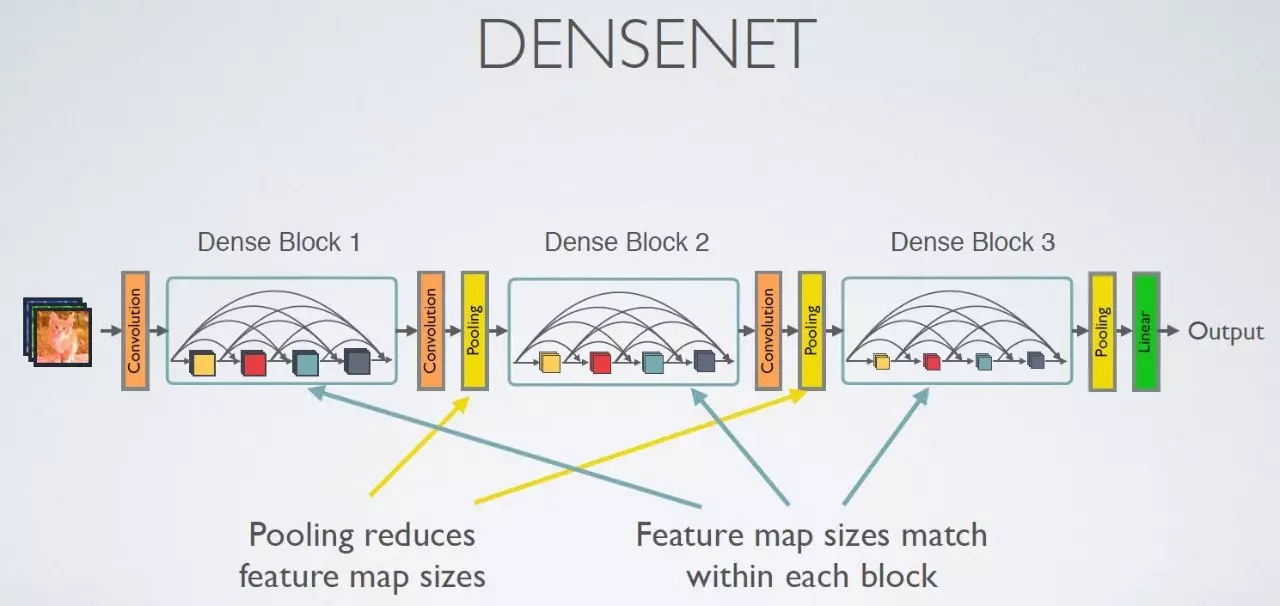
\includegraphics[width=0.6\textwidth]{Densetransferflag0322.png}
\caption{Desnenet结构}
\label{Densetransferflag03220304}
\end{figure}

使用Matlab中的DNN 设计APP可以很快设计出DNN网络 \ref{DNNDesigner20200304}.
%%%%%%%%%%%%%%%%%%%%%%%%%%%%%%%%%%%%%%%%%%
\begin{figure}[H]
\centering
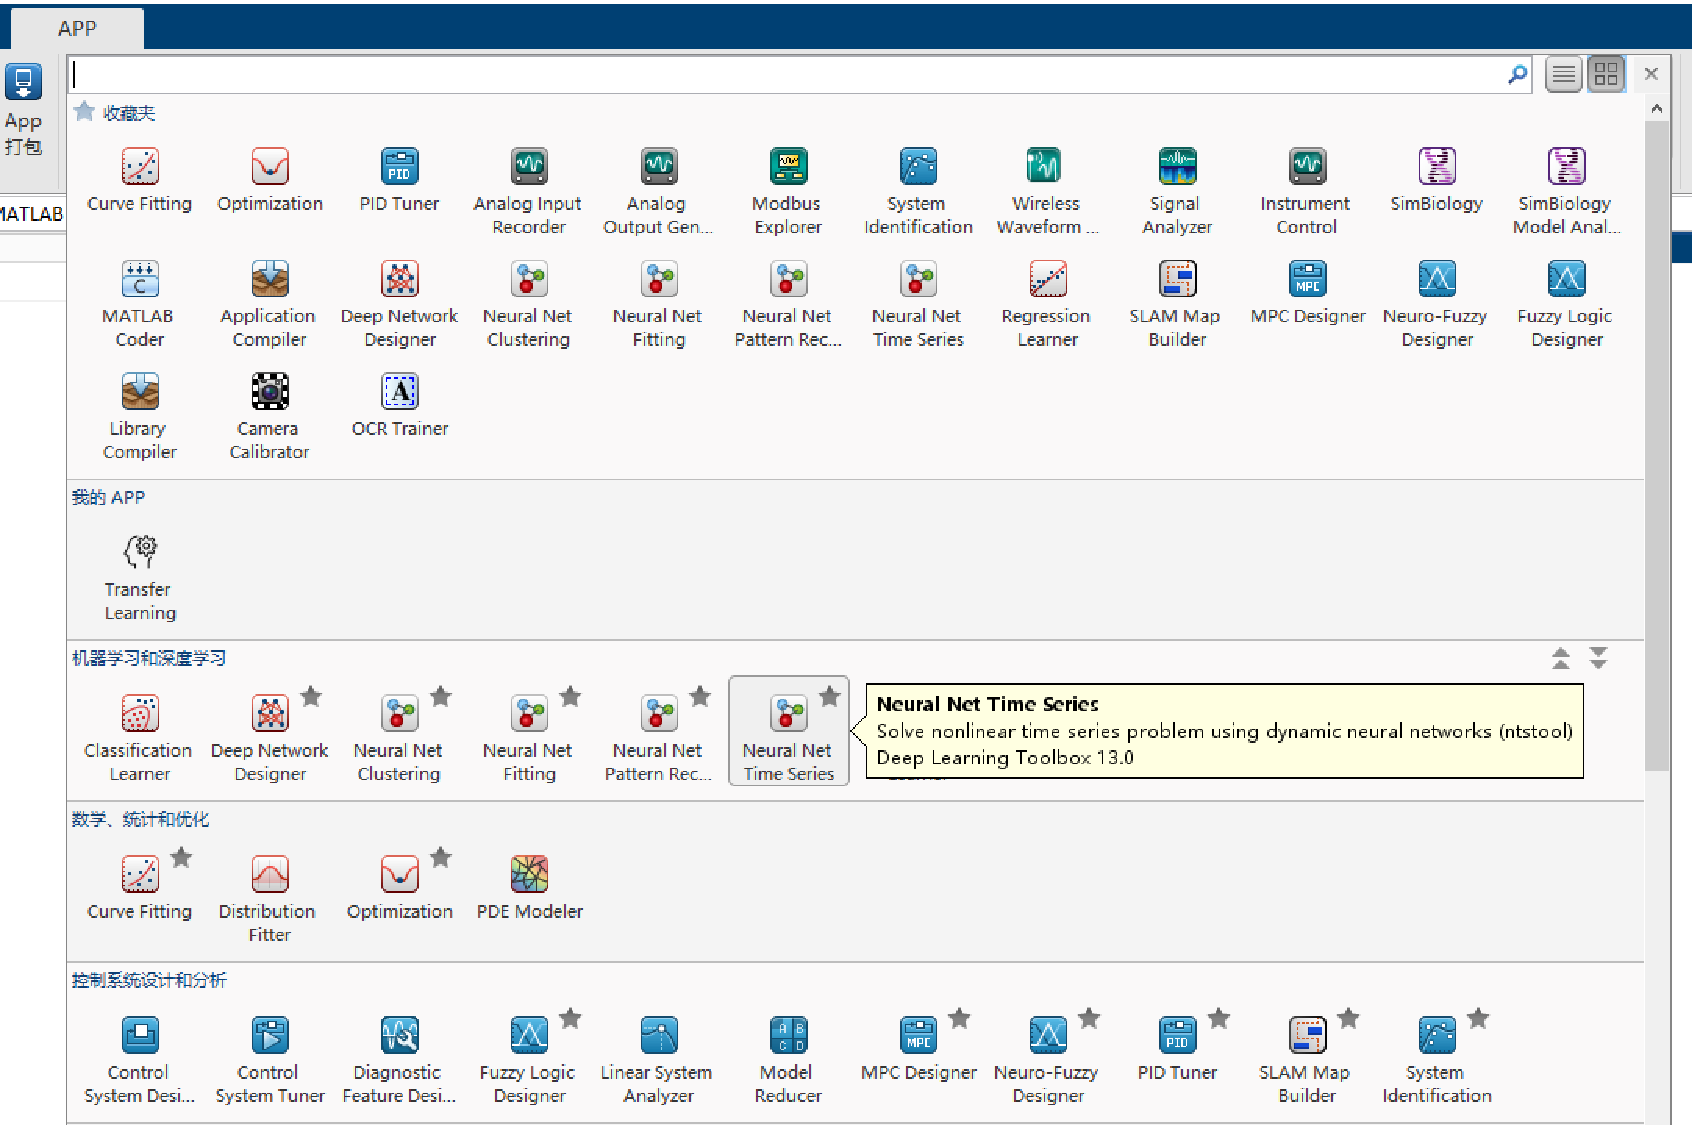
\includegraphics[width=0.5\textwidth]{DNNDesigner.pdf}
\caption{Matlab中的DNN 设计APP}
\label{DNNDesigner20200304}
\end{figure}

%%%%%%%%%%%%%%%%%%%%%%%%%%%%%%%%%%%%%%%%%
\subsection{高速公路网络(Highway network)}
高速公路网络和深度残差学习(DRL)进一步避免了梯度消失, 网络层数达到了前所未有的一百多层(深度残差学习: 152层)\cite{HeCVPR2016-9590, NIPS2015-5850}.
高速公路网络受LSTM门机制的启发, 给网络添加一个传递门和一个搬运门. Highway网络再输入某一层网络的数据一部分经过非线性变换, 另一部分直接从该网络跨过去不做任何转换, 就想走在高速公路上一样, 而多少的数据需要非线性变换, 多少的数据可以直接跨过去, 是由一个权值矩阵和输入数据共同决定的.
\begin{align}
\mathbf{y}=H\left(\mathbf{x}, \mathbf{W}_{\mathbf{H}}\right) \cdot T\left(\mathbf{x}, \mathbf{W}_{\mathbf{T}}\right)+\mathbf{x} \cdot C\left(\mathbf{x}, \mathbf{W}_{\mathbf{C}}\right)
\end{align}
其中$\bm y$向量由两项组成. $T$叫做transform gate, $C$叫做carry gate. $C$和$T$的激活函数都是sigmoid函数.
$T=(b_1, b_2, \cdots, b_n)$,其中每个数字都是$(0, 1)$之间的浮点数, 代表$y$中由$x$变化后的内容所占的比例;
$C=(c_1, c_2, \cdots, c_n)$,其中每个数字也都是$(0, 1)$之间的浮点数, 代表$y$中由$x$本身内容所占的比例;
(为了简便起见, 有时候令$C$可以简化, 取$C=1-T$. $\bm 1$代表了维度和$T$向量样长的单位向量).
需要注意的是, 由于是点乘, 当$C(x,WC)$取了$1-T(x,WT)$之后那么$x,y,H(x,WH),T(x,WT)$必须是同样的维度相容, 以保证可乘.
如果我们想更改$x$的维度变成$B$的维度的话, 一种方法是采用填充零和下采样的方法, 或者是引入一个维度为$A*B$的变换矩阵, 使每次都乘上这个矩阵.

高速公路网络就是在输出和网络层之间加了一个连接, 直接让输入$X$的信息直接通过, 不需要通过神经网络层, 跟高速公路一样.
高速公路网络主要解决的是多层深度神经网络的训练收敛问题, 即使层数很多也可以使用简单的方法比方说反向传播来进行训练, 保证合理的迭代范围内收敛, 而传统的网络是很难保证收敛的. 如图\ref{20170105154423858}所示:
%%%%%%%%%%%%%%%%%%%%%%%%%%%%%%%%%%%%%%%%%%
\begin{figure}[H]
\centering
\includegraphics[width=\textwidth]{20170105154423858.png}
\caption{Highway网络的迭代误差}
\label{20170105154423858}
\end{figure}
当网络很深的时候, 使用了Highway的网络更容易收敛.
%%%%%%%%%%%%%%%%%%%%%%%%%%%%%%%%%%%%%%%%%
\subsection{残差网络}
残差网络用于解决由深度增加而出现错误率增加的情况, 通过拟合残差映射来取代直接的拟合映射.
将一个底层的映射记作 $H(x)$, 用一个堆叠非线性的映射记作 $F(x) = H(x) - x$, 原始的映射变为$F(x) + x$, 我们假设残差映射的优化易于直接映射, 如果某个恒等的映射是最优的, 那么把残差变为0比非线性层的堆叠更简单.
$F(x) + x$ 的形式可以通过前愦神经网络中的快捷连接来实现, 快捷连接 是指跨过或者跳过一定的层, 在这里 shortcut connections 正好实现了identity mapping, 如图\ref{ResidualNND2020202002}
%%%%%%%%%%%%%%%%%%%%%%%%%%%%%%%%%%%%%%%%%%
\begin{figure}[H]
\centering
\includegraphics[width=0.6\textwidth]{ResidualNND2020202002.PNG}
\caption{残差学习网络的结构}
\label{ResidualNND2020202002}
\end{figure}
网络要学习的是$H(x)$, 那么由于图中$\textup{identity} x$之间跨过了2层, 那么其实相当于拟合的是$F(x)=H(x)-x$, 这就是残差概念的来源, 这是论文里的说法.
作者提出的结构打破了传统的神经网络$n-1$层的输出只能给$n$层作为输入的惯例, 使某一层的输出可以直接跨过几层作为后面某一层的输入.
图\ref{DRL2020020301}就是其构造深度残差网络的构思来源图, 一个是56层的网络一个是20层的网络, 从原理上来说其实56层网络的解空间是包括了20层网络的解空间的, 换而言之也就是说, 56层网络取得的性能应该大于等于20层网络的性能的.
但是从训练的迭代过程来看, 56层的网络无论从训练误差来看还是测试误差来看, 误差都大于20层的网络(这也说明了为什么这不是过拟合现象, 因为56层网络本身的训练误差都没有降下去).
导致这个原因就是虽然56层网络的解空间包含了20层网络的解空间, 训练网络用的随机梯度下降策略往往得不到全局最优解, 而是局部的最优解, 显而易见56层网络的解空间更加的复杂, 所以导致使用随机梯度下降算法无法解到最优解.
%%%%%%%%%%%%%%%%%%%%%%%%%%%%%%%%%%%%%%%%%%
\begin{figure}[H]
\centering
\includegraphics[width=0.86\textwidth]{DRL2020020301.PNG}
\caption{CIFAR-10上20层和56层训练误差(左)和测试(右), ImageNet也呈现类似现象}
\label{DRL2020020301}
\end{figure}

在构造这个网络的时候, 如果20层的网络可以取得非常好的结果, 在构造56层网络的时候前20层从20层网络中拷贝过来, 后面的36层只做inentity map至少效果不会差于20层的网络.
于是乎深度残差的网络就提出了, 这个思想其实不复杂, 说白了打破了每一层网络输入只能来自于上一层网络输出的规律, 可以让一些网络的输出直接跳过几层到达后面的输入.
这样的网络确实也取得了非常好的效果. 另外要注意的是, 在真正训练的时候, 有几点小技巧要注意:

1、层与层之间使用批量正则化技术, 否则由于网络过深会导致梯度消失的问题, 导致网络训练无法收敛;

2、为了保持每一层网络的参数差不多, 每当经过了池化层输入的维度减少了一般, 那么滤子的个数就要增加一倍.

其实深度残差网络和Highway网络这两种网络结构都能够让一部分的数据可以跳过某些变换层, 而直接到后面的层中去, 只不过Highway网络需要一个权值来控制每次直接通过的数据量, 而深度残差网络就直接让一部分数据通到了后面.
%%%%%%%%%%%%%%%%%%%%%%%%%%%%%%%%%%%%%%%%%
\section{卷积神经网络 (Convolutional Neural Networks, CNN)}
人工神经网络包括多个神经网络层(卷积层、全连接层、LSTM等), 每一层又包括很多神经元, 超过三层的非线性神经网络都可以被成为深度神经网络.
神经网络允许机器通过识别可以广泛应用的模式来学习, 其应用包括语言识别、视觉物体识别、自动驾驶汽车导航, 机械臂的灵活抓取等. 作为一个科学领域, 神经网络的发端可以追溯到上世纪 40 年代, 但直到最近几年, 该领域才取得了显著进展.
通俗的讲, 深度学习的模型可以视为是输入到输出的映射函数, 比如中文到英文的映射, 足够深的神经网络理论上可以拟合任何复杂的函数
“深度”是指网络中的层数 — 层数越多, 网络越深. 传统的神经网络只包含 2 层或 3 层, 而深度网络可能有几百层.
深度学习是机器学习的一个类型, 该类型的模型直接从图像、文本或声音中学习执行分类任务. 通常使用神经网络架构实现深度学习.
深度学习由一连串可微分的参数化的层组成, 而且是用反向传播算法端到端地训练的.
\begin{remark}
\textbf{深度学习领域被引最高的论文}:
神经网络实际上是一个泛逼近器. 用形象点的类比来说, 可以把神经网络视为一个超级大的万能工匠玩具——大量互相连接的节点阵列, 可以训练来完成许多任务, 从语言翻译到识别物体、识别人类讲话.
作为“LSTM 之父”的 Jürgen Schmidhuber 在深度学习领域的贡献仍然获得了整个社区的认可.
Google Scholar 2019年统计发现:  Hochreiter 和 Schmidhuber 1997 年发表的 LSTM 论文成为了20世纪被引最高的深度学习研究论文\cite{HochreiterNC1997}.
\end{remark}

François Chollet, Keras作者、谷歌大脑高级研究员 François Chollet的观点: 深度学习应该指的是一种表征学习方法, 其中的模型是由一连串的模块组成的(一般都会堆成一个多层的或者金字塔形的模型, 这也就是「深度」的由来), 而其中的每一个模块分别拿出来训练之后都可以作为独立的特征提取器. CNN 专门解决图像问题的特征提取.
\begin{example}
  如果你有一个卷积网络模型, 然后你用 ADMM 训练它的权重, 它就不是深度学习了吗?一个自己学习特征的 HMAX 模型就不是深度学习了吗?甚至于, 用贪婪算法逐层训练的深度神经网络就不是深度学习了吗?要我说的话, 它们都是深度学习.
\end{example}

深度学习中的 AlexNet一开始有 8层网络, 约 6000万个参数; 发展到 2014 年的 VGG-19模型, 有 19 层网络, 大概 1.43 亿个参数, 深度学习模型越来越复杂, 如果无法直接在存储中处理数据和模型, 就会对带宽造成巨大堵塞, 对效率产生很大影响.
这就要求提高边缘端的计算能力, 主要的推进方向有两个:  一是从神经网络模型的表示、计算、存储、 和学习等方面, 通过压缩、剪枝、量化等方法来简化模型;  二是使用专用加速器加速深度学习应用, 将 32bits 浮点数转换为定点数, 减少延迟, 降低能耗.
深度学习常用的神经网络算法图\ref{DNN191218121500010}-图\ref{DNN191218121500011}. CNN相对于DNN, 比较特殊的是卷积层和池化层, 在熟悉DNN的基础上, 理解卷积层和池化层的原理就学会了CNN.

%%%%%%%%%%%%%%%%%%%%%%%%%%%%%%%%%%%%%%%%%
深度学习在神经网络研究者中间已经被讨论了超过二十年. 最近深度学习的发展是由相对较小的算法改进以及大数据集模型和计算机硬件发展驱动的.
深度学习是一种特定形式的机器学习, 训练多层神经网络. 深度学习近年来非常流行, 引领了图像识别和语音识别等领域的突破性进展. (Stuart Russell: 人工智能基础概念与34个误区.)
深度学习已经代替了机器学习的地位.
%%%%%%%%%%%%%%%%%%%%%%%%%%%%%%%%%%%%%%%%%%
\begin{figure}[H]
\centering
\includegraphics[width=0.86\textwidth]{DNN1912181.png}
\caption{DNN的各种结构(2)}
\label{DNN191218121500011}
\end{figure}
%%%%%%%%%%%%%%%%%%%%%%%%%%%%%%%%%%%%%%%%%%
\begin{figure}[H]
\centering
\includegraphics[width=0.76\textwidth]{lstm20191229085814.png}
\caption{LSTM结构}
\label{lstm20191229085814}
\end{figure}
%%%%%%%%%%%%%%%%%%%%%%%%%%%%%%%%%%%%%%%%%
CNN是第一个真正成功训练多层网络结构的学习算法. 它利用局部连接, 权重共享和下采样极大降低了模型的参数数量, 以提高一般BP网络的训练性能.
在CNN中, 图像的一小部分(局部感受区域)作为层级结构的最低层的输入, 神经元只与上一层中部分神经元相连, 并且不同的神经元共享权值, 每层通过不同的卷积核去获得观测数据的不同特征, 然后通过下采样(池化)将语义上相似的特
征合并起来, 降低特征图的空间分辨率.  CNN能够提取对平移、缩放和旋转不变的观测数据的显著特征, 在图像处理、语音处理等领域得到了广泛而深入的应用.
%%%%%%%%%%%%%%%%%%%%%%%%%%%%%%%%%%%%%%
\paragraph{CNN应用场景——计算机视觉问题}

\ding{172} 图像分类( Classification) : 识别出该图像属于哪个类别.

\ding{173} 目标定位( Localization) :  在图像分类的基础上,  定位找到对象在图像中的位置.

\ding{174} 目标检测( Detection) : 给出在图像内所有该类别的目标和对应的位置.

\ding{175} 图像分割( Segmentation) : 具体到像素级别的图像处理.

\ding{176} 无人驾驶汽车在接近人行横道线时减速.

\ding{177} ATM 拒收假钞.

\ding{178} 智能手机应用程序即时翻译国外路标.

\ding{179} UCLA 研究人员建造了一种高级显微镜, 能产生高维的数据集, 用来训练深度学习网络, 在组织检体中识别癌细胞.

深度学习特别适合鉴别应用场景, 比如人脸辨识、文本翻译、语音识别以及高级驾驶辅助系统(包括车道分类和交通标志识别).
先进的工具和技术极大改进了深度学习算法, 达到了很高的水平, 在图像分类上能够超越人类, 能打败世界最优秀的围棋选手, 还能实现语音控制助理功能, 如 Amazon Echo® 和 Google Home, 可用来查找和下载您喜欢的新歌.

三个技术助推器让这种精确度成为可能:
\begin{itemize}
\item 大规模带标签的数据集ImageNet 和 PASCAL VoC 等数据集可以免费使用, 对于许多不同类型的对象训练十分有用.
%%%%%%%%%%%%%%%%%%%%%%%%%%%%%%%%%%%%%%%%%%
\begin{figure}[H]
\centering
\includegraphics[width=0.76\textwidth]{DNNUlabelSet.JPG}
\caption{大规模带标签的免费数据集}
\label{DNNUlabelSet201912250001}
\end{figure}
\item 增大的计算能力: 高性能 GPU 加快了深度学习所需的海量数据的训练速度, 训练时间从几星期减少到几小时.
%%%%%%%%%%%%%%%%%%%%%%%%%%%%%%%%%%%%%%%%%%
\begin{figure}[H]
\centering
\includegraphics[width=0.76\textwidth]{GPUCloud.JPG}
\caption{算力的规模}
\label{GPUCloud201912250002}
\end{figure}
\item 由专家构建的预先训练好的模型可以重新训练 AlexNet之类的模型, 使用名为迁移学习的技术执行新识别任务. 虽然使用了 130万张高分辨率图像训练 AlexNet来识别 1000个不同的对象, 但可以使用较小的数据集实现精确的迁移学习.
\end{itemize}
%%%%%%%%%%%%%%%%%%%%%%%%%%%%%%%%%%%%%%%%%%
\begin{figure}[H]
\centering
\includegraphics[width=0.76\textwidth]{AleNet130.JPG}
\caption{迁移学习模型}
\label{AleNet130201912250003}
\end{figure}
%%%%%%%%%%%%%%%%%%%%%%%%%%%%%%%%%%%%%%%%%%
\begin{figure}[H]
\centering
\includegraphics[width=0.76\textwidth]{CNNAPP201912150001.PNG}
\caption{ AlexNet的目标分割}
\label{CNNAPP201912150001}
\end{figure}
%%%%%%%%%%%%%%%%%%%%%%%%%%%%%%%%%%%%%%%%%%
\begin{figure}[H]
\centering
\includegraphics[width=0.76\textwidth]{DNN191225001.JPG}
\caption{深度神经网络}
\label{DNN191225001}
\end{figure}
%%%%%%%%%%%%%%%%%%%%%%%%%%%%%%%%%%%%%%%%%%%%%%%%%
\subsection{卷积神经网络结构}
传统的CNN网络只能给出图像的LABLE, 但是在很多情况下需要对识别的物体进行首尾相连地分割, FCN的出现给物体分割提供了一个非常重要的解决思路, 其核心就是卷积与反卷积.
%%%%%%%%%%%%%%%%%%%%%%%%%%%%%%%%%%%%%%%
\subsubsection{卷积}
对于1维的卷积, 离散公式与连续计算过程如下, 要记住的是原函数或者卷积函数在卷积前要翻转180度.
%%%%%%%%%%%%%%%%%%%%%%%%%%%%%%%%%%%%%%%%%
\begin{figure}[H]
\centering
\animategraphics[width=0.86\textwidth,autoplay,controls]{2}{ConvolutionOP0203}{1}{301}
\caption{1维离散卷积公式的计算过程}
\label{ConvolutionOP0203}
\end{figure}

对于离散卷积, $f$的大小是$n_1, g$的大小是$n_2$, 卷积后的大小是$n_1+n_2-1$.
同样地, 卷积的计算需要对卷积核进行180的旋转, 同时卷积核中心与需要计算的图像像素对齐, 输出结构为中心对齐像素的一个新的像素值.
%%%%%%%%%%%%%%%%%%%%%%%%%%%%%%%%%%%%%%%%%%
\begin{example}
计算出图\ref{JuanJi2020020301}左上角(即第一行第一列)像素的卷积后像素值, 其中
\begin{figure}[H]
\centering
\includegraphics[width=0.65\textwidth]{TUCon2020020302.PNG}
\caption{输入和卷积核}
\label{TUCon2020020302}
\end{figure}
\begin{figure}[H]
\centering
\includegraphics[width=0.3\textwidth]{JuanJi2020020301.PNG}
\caption{第一行第一列像素值}
\label{JuanJi2020020301}
\end{figure}
像素左上角位置记为$[0,0]$, 图像值为1; $h$为卷积核, $x$为图像值, 不足的填充0.
$$
\begin{aligned}
y[0,0]=& x[-1,-1] \cdot h[1,1]+x[0,-1] \cdot h[0,1]+x[1,-1] \cdot h[-1,1] \\
       &+x[-1,0] \cdot h[1,0]+x[0,0] \cdot h[0,0]+x[1,0] \cdot h[-1,0] \\
       &+x[-1,1] \cdot h[1,-1]+x[0,1] \cdot h[0,-1]+x[1,1] \cdot h[-1,-1] \\
      =&[0,0,0]\cdot [1,2,1]^T+[0,1,2]\cdot [0,0,0]^T+[0,4,5]\cdot [-1,-2,-1]^T\\
      =& 0\cdot 1+0 \cdot 2+0 \cdot 1+0 \cdot 0+1 \cdot 0+2 \cdot 0+0 \cdot(-1)+4 \cdot(-2)+5 \cdot(-1)\\
      =&-13.
\end{aligned}$$
通过滑动卷积核, 就可以得到整张图片的卷积结果(图\ref{TUCon2020020302}的输出), 可以看出, 通过图像卷积后的新图像大小跟原来一样甚至变小.
\end{example}

%%%%%%%%%%%%%%%%%%%%%%%%%%%%%%%%%%%%%%%%%%%%%%%%%%
\begin{example}
从左到右运算后, 原像素经过卷积由$1$变成$-8$(图\ref{CNN20161021131748099}).
%%%%%%%%%%%%%%%%%%%%%%%%%%%%%%%%%%%%%%%%%%
\begin{figure}[H]
\centering
\includegraphics[width=0.6\textwidth]{20161021131748099.png}
\caption{卷积核对图像逐像素点运算}
\label{CNN20161021131748099}
\end{figure}
\end{example}

图\ref{TUCon2020020302}经过same卷积计算后图像大小不变. 图\ref{CNN20161021131748099}卷积计算后图像大小不变. 图\ref{20161021135241205}经过valid卷积后图像变小, 是因为没有对所用像素进行卷积计算.
%%%%%%%%%%%%%%%%%%%%%%%%%%%%%%%%%%%%%%%%%
\begin{figure}[H]
\centering
\animategraphics[width=0.4\textwidth,autoplay,controls]{2}{20161021135241205}{1}{9}
\caption{valid卷积运算}
\label{20161021135241205}
\end{figure}

\href{https://cn.mathworks.com/help/matlab/ref/conv2.html?requestedDomain=www.mathworks.com}{Matlab}中2维卷积分为完全卷积、same卷积和valid卷积.
2维完全卷积如图\ref{CNN20161021141659634}.
图\ref{CNN20161021141659634}中蓝色区域是原图像, 白色为对应卷积所增加的填充, 通常的填充全部为0, 绿色是卷积后图片.
卷积的滑动是从\uwave{卷积核右下角与图片左上角重叠开始进行卷积}, 滑动步长为1, 卷积核的中心元素对应卷积后图像的像素点.
可以看到卷积后的图像是$4\times 4$, 比原图$2\times 2$大, 记1维卷积大小是$n_1+n_2-1$, 这里原图是$2\times 2$, 卷积核$3\times 3$, 卷积后结果是$4\times 4$, 与一维完全对应起来,
$4\times 4$的卷积是完整的卷积计算. 其他比它小的卷积结果都是省去了部分像素的卷积.
%%%%%%%%%%%%%%%%%%%%%%%%%%%%%%%%%%%%%%%%%%
\begin{figure}[H]
\centering
\animategraphics[width=0.4\textwidth,autoplay,controls]{2}{CNN20161021141659634}{1}{16}
\caption{2维完全卷积}
\label{CNN20161021141659634}
\end{figure}
对应图像卷积后多出部分的解释(来自WIKI): 多出来的部分根据实际情况可以有不同的处理方法(这里的full卷积就是后面要说的反卷积),
我们可以对卷积核移动范围的不同限制, 得到full卷积, same卷积 (指经过卷积的特征图和原图的size保持不变), valid卷积(滤镜全部在image里面的时候, 进行卷积运算, 可见滤镜的移动范围较same卷积更小), 三种卷积后图像大小的计算公式:

1) full卷积: 滑动步长为1, 图片大小为$N_1\times N_1$, 卷积核大小为$N_2\times N_2$, 卷积后图像大小:$(N_1+N_2-1) \times (N_1+N_2-1)$.
如图 \ref{CNN20161021141659634}, 滑动步长为1, 图片大小为$2\times 2$, 卷积核大小为$3\times 3$, 卷积后图像大小:$4\times 4$.

2) same卷积: 滑动步长为1, 图片大小为$N_1\times N_1$, 卷积核大小为$N_2\times N_2$, 卷积后图像大小: $N_1\times N_1$.

3) valid卷积: 滑动步长为S, 图片大小为$N_1\times N_1$, 卷积核大小为$N_2\times N_2$, 卷积后图像大小:$((N_1-N_2)/S+1) \times ((N_1-N_2)/S+1)$.
如图 \ref{20161021135241205}, 滑动步长为1, 图片大小为$5\times 5$, 卷积核大小为$3\times 3$, 卷积后图像大小: $3\times 3$.

%%%%%%%%%%%%%%%%%%%%%%%%%%%%%%%%%%%%%%%
\subsubsection{反卷积(后卷积, 转置卷积)}

反卷积跟1维信号处理的反卷积计算不一样, FCN作者称为后向卷积层, 有人称反卷积层应该称为转移卷积层.
CNN中有卷积层与池化层, 卷积层进行对图像卷积提取特征, 池化层对图像缩小一半筛选重要特征, 对于经典的图像识别CNN网络, 如IMAGENET, 最后输出结果是$1\times 1\times 1000$, 1000是类别种类.
FCN作者和后来的研究人员都对最终$1\times 1$的结果使用反卷积(事实上FCN作者最后的输出不是$1\times 1$, 是图片大小的32分之一, 但不影响反卷积的使用).
%%%%%%%%%%%%%%%%%%%%%%%%%%%%%%%%%%%%%%%%%%
\begin{example}
大小为$2\times 2$图像的反卷积过程如图\ref{20170715175257862}, 其中输入$2\times 2$, 卷积核$4\times 4$, 滑动步长3, 输出$7\times 7$, 图\ref{20170715175257862}给出了输入为$2\times 2$的图片经过$4\times 4$的卷积核进行步长为3的反卷积运算过程.
1) 输入图片每个像素进行一次full卷积, 根据full卷积大小计算可以知道每个像素的卷积后大小为 $1+4-1=4$,  即$4\times 4$大小的特征图, 输入有4个像素所以4个$4\times 4$的特征图.

2) 将4个特征图进行步长为3的融合(即相加); 例如红色的特征图仍然是在原来输入位置(左上角), 绿色还是在原来的位置(右上角), 步长为3是指每隔3个像素进行融合, 重叠部分进行相加, 即输出的第1行第4列是由红色特阵图的第一行第四列与绿色特征图的第一行第一列相加得到, 其他如此类推.

可以看出反卷积的大小是由卷积核大小与滑动步长决定, in是输入大小, $k$是卷积核大小, $s$是滑动步长, out是输出大小.
得到 $\textup{out} = (\textup{in} - 1) * s + k$, 图\ref{20170715175257862}过程就可以写为$(2 - 1)\times 3 + 4 = 7$.
\begin{figure}[H]
\centering
\includegraphics[width=0.86\textwidth]{20170715175257862.png}
\caption{大小为$2\times 2$图像的反卷积过程}
\label{20170715175257862}
\end{figure}
\end{example}
这种反卷积的使用使得图像可以变大, FCN作者使用的方法是这里所说反卷积的一种变体, 这样就可以获得相应的像素值, 图像可以实现首尾相连地分割. 图像的反卷积见图 \ref{Dconop0203}的\href{https://github.com/vdumoulin/conv_arithmetic}{full卷积原理}.
%%%%%%%%%%%%%%%%%%%%%%%%%%%%%%%%%%%%%%%%%%
\begin{figure}[H]
\centering
\animategraphics[width=0.45\textwidth,autoplay,controls]{2}{Dconop0203}{1}{25}
\caption{反卷积运算}
\label{Dconop0203}
\end{figure}
%%%%%%%%%%%%%%%%%%%%%%%%%%%%%%%%%%%%%%%
\subsubsection{卷积神经网络的层结构}
卷积神经网络(CNN 或 ConvNet)是图像和视频深度学习的最流行算法之一.
像其他神经网络一样, CNN 由一个输入层、一个输出层和中间的多个隐藏层组成.
\begin{itemize}
\item 特征检测层: 这些层对数据执行三种类型操作中的一种, 即卷积、池化或修正线性单元 (ReLU, 图\ref{ReLU20200203001}).
%%%%%%%%%%%%%%%%%%%%%%%%%%%%%%%%%%%%%%%%%%
\begin{figure}[H]
\begin{center}
\begin{tikzpicture}
    \begin{axis}[
        domain=-3:5,
        ]
        \addplot+[mark=none,red,domain=-3:0] {0};
        \addplot+[mark=none,red,domain=0:5] {x};
    \end{axis}
\end{tikzpicture}
% 另一种方式
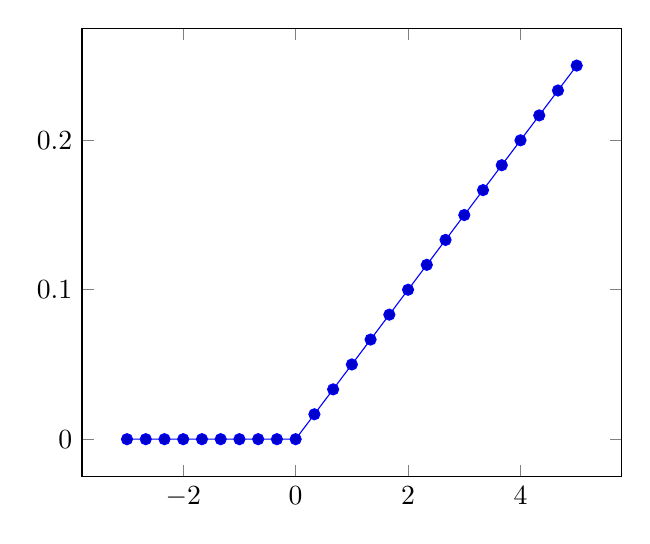
\begin{tikzpicture}
        \begin{axis}[
            domain=-3:5,
        ]
            \addplot {
                ifthenelse(
                    x<0,        % if
                    0,          % then
                    0.05*x           % else
                )
            };
        \end{axis}
    \end{tikzpicture}
\end{center}
\caption{修正线性单元和$\alpha=0.05$的leaky修正线性单元}
\label{ReLU20200203001}
\end{figure}

\item \textbf{卷积}将输入图像放进一组卷积过滤器, 每个过滤器激活图像中的某些特征.
\item \textbf{池化}通过执行非线性下采样, 减少网络需要学习的参数个数, 从而简化输出.
\item \textbf{修正线性单元} (ReLU) 通过将负值映射到零和保持正数值, 实现更快、更高效的训练.
\end{itemize}

这三种操作在几十层或几百层上反复进行, 每一层都学习检测不同的特征.
%%%%%%%%%%%%%%%%%%%%%%%%%%%%%%%%%%%%%%%
\subsubsection{激活函数和层范数}
\href{https://dashee87.github.io/deep\%20learning/visualising-activation-functions-in-neural-networks/}{在线绘制 各类激活函数}.
\begin{remark}
Leaky ReLU激活函数是在声学模型(2013)中提出的, 给所有负值赋予一个非零斜率$\alpha=\frac 1 {a_i}, a_i\in (1,\infty)$.
\end{remark}
\begin{remark}
CELU \cite{hendrycks2016gelu} 定义为
\begin{align}
 CELU(x)=\max(0,x)+\min(0,\alpha(\exp(x/\alpha)-1)), x\in \mathbb R, \alpha> 0.
\end{align}
\end{remark}
\begin{remark}
高斯线性误差单元 (GELU), 是高性能神经网络的一种激活函数. GELU的非线性体现在它的随机正则化算子会随机地应用恒等映射和零映射到神经元的输入上.
GELU的非线性权重输入由幅值决定, 不同于ReLUs中由符号决定.
\begin{align}
  \operatorname{GELU}(x)=x P(X \leq x)=x \Phi(x)
\end{align}
使用下式可以逼近GELU
\begin{align}
  0.5 x\left(1+\tanh \left[\sqrt{2 / \pi}\left(x+0.044715 x^{3}\right)\right]\right)
\end{align}
或者
\begin{align}
  x \sigma(1.702 x).
\end{align}
\end{remark}

Bent-identity
\begin{align}
  f(x) = \frac{\sqrt{x^2 + 1} - 1}{2} +x
\end{align}

Synthesization of many useful properties of other activations, including PReLU, ELU, and SELU and CIFAR -10 experiments  validation \cite{Godfrey2019-9846}, 2019 IEEE International Conference on Systems, Man and Cybernetics (SMC), 6-9 Oct. 2019.

Rothaus在1976年提出.因为Bent函数既是非线性度最优的布尔函数, 介于 Identity 与 ReLU之间的一种折衷选择. 它允许非线性行为, 尽管其非零导数有效提升了学习并克服了与 ReLU相关的静默神经元的问题.
由于其导数可在 1 的任意一侧返回值, 因此它可能容易受到梯度爆炸和消失的影响.

\href{https://arxiv.org/pdf/1901.05894.pdf}{LiSHT (Linearly Scaled Hyperbolic Tangent) function}:
\begin{align}
  \phi(x)=x \cdot g(x), g(x)=\operatorname{Tanh}(x)=\frac{\exp ^{x}-\exp ^{-x}}{\exp ^{x}+\exp ^{-x}}
\end{align}



Swish activation function \cite{Ramachandran2018}
\begin{align}
  y(x)=x /\left(1+e^{-x}\right).
\end{align}

\href{https://arxiv.org/pdf/1808.00783.pdf}{ELiSH-\href{https://workshops.aapr.at/wp-content/uploads/2019/05/ARW-OAGM19_41.pdf}{The Quest for the Golden Activation Function}: Proceedings of the ARW \& OAGM Workshop 2019, May 9-10, 2019 in Steyr, Austria}(Exponential Linear Sigmoid SquasHing)

A piecewise activation function, which shares the goodness of Swish in positive part \& ELU and Sigmoid in its negative part.
In Swish, Sigmoid improves the information flow and Linear avoids a vanishing gradient, which is also the main motivation to design ELiSH.
\begin{align}
    y(x)=\left\{\begin{array}{ll}
    x /\left(1+e^{-x}\right) & x \geq 0 \\
    \left(e^{x}-1\right) /\left(1+e^{-x}\right) & x<0
    \end{array}\right.
\end{align}
HardELiSH as a multiplication of HardSigmoid and ELU in negative part and HardSigmoid and Linear in positive part
\begin{align}
    y(x)=\left\{\begin{array}{ll}
    x \times \max (0, \min (1,(x+1) / 2)) & x \geq 0 \\
    \left(e^{x}-1\right) \times \max (0, \min (1,(x+1) / 2)) & x<0
    \end{array}\right.
\end{align}

Soft shrinkage function elementwise:
\begin{align}
\text { Soft Shrinkage }(x)=\left\{\begin{array}{ll}
{x-\lambda,} & {\text { if } x>\lambda} \\
{x+\lambda,} & {\text { if } x<-\lambda} \\
{0,} & {\text { otherwise }}
\end{array}\right.
\end{align}
参数默认是$\lambda=0.5$.

Softsign

\begin{align}
  \operatorname{Soft} \operatorname{Sign}(x)=\frac{x}{1+|x|}
\end{align}

Tanhshrink

\begin{align}
  \operatorname{Tanhshrink} (x)=x- \operatorname{Tanh} (x).
\end{align}

Softmin

\begin{align}
 \operatorname{Softmin}\left(x_{i}\right)=\frac{\exp \left(-x_{i}\right)}{\sum_{j} \exp \left(-x_{j}\right)}
\end{align}

Softmax

\begin{align}
  \operatorname{Softmax}\left(x_{i}\right)=\frac{\exp \left(x_{i}\right)}{\sum_{j} \exp \left(x_{j}\right)}
\end{align}

LogSoftmax

\begin{align}
  \log \operatorname{Softmax}\left(x_{i}\right)=\log \left(\frac{\exp \left(x_{i}\right)}{\sum_{j} \exp \left(x_{j}\right)}\right)
\end{align}


\href{https://pytorch.org/docs/stable/nn.html#torch.nn.Softshrink}{AdaptiveLogSoftmaxWithLoss}

\begin{align}
  y=\frac{x-\mathrm{E}[x]}{\sqrt{\mathrm{Var}[x]+\epsilon}} * \gamma+\beta
\end{align}

BatchNorm1d

\begin{align}
y=\frac{x-\mathrm{E}[x]}{\sqrt{\mathrm{Var}[x]+\epsilon}} * \gamma+\beta
\end{align}

BatchNorm2d

\begin{align}
  y=\frac{x-\mathrm{E}[x]}{\sqrt{\operatorname{Var}[x]+\epsilon}} * \gamma+\beta
\end{align}

BatchNorm3d

\begin{align}
  y=\frac{x-\mathrm{E}[x]}{\sqrt{\mathrm{Var}[x]+\epsilon}} * \gamma+\beta
\end{align}


GroupNorm

\begin{align}
  y=\frac{x-\mathrm{E}[x]}{\sqrt{\mathrm{Var}[x]+\epsilon}} * \gamma+\beta
\end{align}

SyncBatchNorm

\begin{align}
  y=\frac{x-\mathrm{E}[x]}{\sqrt{\mathrm{Var}[x]+\epsilon}} * \gamma+\beta
\end{align}

InstanceNorm1d

\begin{align}
  y=\frac{x-\mathrm{E}[x]}{\sqrt{\operatorname{Var}[x]+\epsilon}} * \gamma+\beta
\end{align}

SoftExponential
\begin{align}
  f(\alpha, x)=\left\{\begin{array}{ll}
{-\frac{\ln (1-\alpha(x+\alpha))}{\alpha}} & {\text { for } \alpha<0} \\
{x} & {\text { for } \alpha=0} \\
{\frac{e^{\alpha x}-1}{\alpha}+\alpha} & {\text { for } \alpha>0}
\end{array}\right., x\in (-\infty, \infty)
\end{align}

InstanceNorm3d

\begin{align}
  y=\frac{x-\mathrm{E}|x|}{\sqrt{\mathrm{Var}[x]+\epsilon}} * \gamma+\beta
\end{align}

LayerNorm

\begin{align}
  y=\frac{x-\mathrm{E}[x]}{\sqrt{\mathrm{Var}[x]+\epsilon} * \gamma+\beta}
\end{align}

LocalResponseNorm

\begin{align}
  b_{c}=a_{c}\left(k+\frac{\alpha}{n} \sum_{c^{\prime}=\max (0, c-n / 2)}^{\min (N-1, c+n / 2)} a_{c^{\prime}}^{2}\right)^{-\beta}
\end{align}

\href{http://www.gabormelli.com/RKB/Inverse_Square_Root_Unit_(ISRU)_Activation_Function}{ISRU (Inverse Square Root Unit)} \cite{BradCarlile2017}
\begin{align}
  f(x)=\frac{x}{\sqrt{1+\alpha x^{2}}}, x\in \left(-\frac{1}{\sqrt{\alpha}}, \frac{1}{\sqrt{\alpha}}\right)
\end{align}

Inverse square root linear unit (ISRLU) \cite{BradCarlile2017}
\begin{align}
f(x)=\left\{\begin{array}{ll}
{\frac{x}{\sqrt{1+\alpha x^{2}}}} & {\text { for } x<0} \\
{x} & {\text { for } x \geq 0}
\end{array}\right., x\in \left(-\frac{1}{\sqrt{\alpha}}, \infty\right)
\end{align}

SoftPlus \cite{glorot2011}
\begin{align}
  f(x)=\ln \left(1+e^{x}\right), x\in (0, \infty)
\end{align}

Multi-layer long short-term memory (LSTM) RNN to an input sequence.
\begin{align}
\begin{array}{l}
{i_{t}=\sigma\left(W_{i i} x_{t}+b_{i i}+W_{h i} h_{(t-1)}+b_{h i}\right)} \\
{f_{t}=\sigma\left(W_{i f} x_{t}+b_{i f}+W_{h f} h_{(t-1)}+b_{h f}\right)} \\
{g_{t}=\tanh \left(W_{i g} x_{t}+b_{i g}+W_{h g} h_{(t-1)}+b_{h g}\right)} \\
{o_{t}=\sigma\left(W_{i o} x_{t}+b_{i o}+W_{h o} h_{(t-1)}+b_{h o}\right)} \\
{c_{t}=f_{t} * c_{(t-1)}+i_{t} * g_{t}} \\
{h_{t}=o_{t} * \tanh \left(c_{t}\right)}
\end{array}
\end{align}
where $h_t$ is the hidden state at time $t$, $c_t$ is the cell state at time $t$, $x_t$ is the input at time $t$, $h_{(t-1)}$ is the hidden state of the layer at time $t-1$ or the initial hidden state at time 0,
and $i_t$, $f_t, g_t, o_t$ are the input, forget, cell, and output gates, respectively. $\sigma$ is the sigmoid function, and $*$ is the Hadamard product.
%%%%%%%%%%%%%%%%%%%%%%%%%%%%%%%%%%%%%%%%%%
\begin{figure}[H]
\centering
\includegraphics[width=0.76\textwidth]{CNNStructure1225001.JPG}
\caption{卷积神经网络}
\label{CNNStructure1225001}
\end{figure}

\textbf{分类层}在特征检测之后, CNN 的架构转移到分类. 倒数第二层是全连接层 (FCL), 输出$K$维度的向量, 其中$K$是网络能够预测的类数量. 此向量包含任何图像的每个类进行分类的概率. CNN 架构的最后一层使用 softmax 函数提供分类输出.

没有用于选择层数的确切公式. 最好的方法是尝试一些层, 查看工作效果如何, 或者使用预先训练好的网络.
%%%%%%%%%%%%%%%%%%%%%%%%%%%%%%%%%%%%%%%%%%
\begin{figure}[H]
\centering
\includegraphics[width=0.76\textwidth]{CNNStructure1225002.JPG}
\caption{卷积神经网络}
\label{CNNStructure1225002}
\end{figure}

深度学习是机器学习的子类型. 使用机器学习, 您手动提取图像的相关特征. 使用深度学习, 您将原始图像直接馈送给深度神经网络, 该网络自动学习特征.
为了获得最佳结果, 深度学习通常需要成百上千乃至数百万张图像. 而且属于计算密集型, 需要高性能 GPU.
%%%%%%%%%%%%%%%%%%%%%%%%%%%%%%%%%%%%%%%%%%
\begin{figure}[H]
\centering
\includegraphics[width=0.6\textwidth]{AlexNetdemo002.JPG}
\caption{AlexNet的识别对象}
\label{AlexNetdemo002}
\end{figure}
刚接触深度学习, 快速而轻松的入门方法是使用现有网络, 比如 2012 年首次发布的AlexNet, 已成为研究团体中众所周知的模型. 用一百多万张图像训练好的 CNN.  AlexNet 最常用于
图像分类. 它可将图像划分为 1000 个不同的类别, 包括键盘、鼠标、铅笔和其他办公设备, 以及各个品种的狗、猫、马和其他动物.
%%%%%%%%%%%%%%%%%%%%%%%%%%%%%%%%%%%%%%%%%%
\begin{figure}[H]
\centering
\includegraphics[width=0.76\textwidth]{CNNMLCompare001.JPG}
\caption{机器学习和深度学习}
\label{CNNMLCompare001}
\end{figure}
%%%%%%%%%%%%%%%%%%%%%%%%%%%%%%%%%%%%%%%%%%%%
\begin{example}
(\textbf{AlexNet 的Matlab示例}) 使用 AlexNet 对任何图像中的对象分类. 在本例中, 我们使用它对桌上安装的网络摄像头捕获的图像中的对象分类. 除了 MATLAB, 我们还使用下列工具:
\begin{itemize}
\item Deep Learning Toolbox™;
\item 在 MATLAB 中使用网络摄像头的支持包;
\item 使用 AlexNet 的支持包.
\end{itemize}
在加载 AlexNet 后, 我们连接到网络摄像头并拍摄一张实时图像.
\begin{Verbatim}
camera = webcam; % 连接到摄像头
nnet = AlexNet; % 加载神经网络
picture = camera.snapshot;
% 抓取图片
\end{Verbatim}
接下来, 我们调整图像大小为 227x227 像素, 即 AlexNet所需的大小.
\begin{Verbatim}
picture = imresize(picture,[227,227]);
% 调整图片大小
AlexNet 现在可对我们的图像分类.
label = classify(nnet, picture);
% 对图片分类
image(picture); % 显示图片
title(char(label)); % 显示标签
\end{Verbatim}
\end{example}
上一示例使用的是现成的网络. 我们完全不做任何修改, 因为 AlexNet 训练所用的图像类似于我们想要分类的图像.

要使用 AlexNet 对未在原有网络中训练的对象分类, 我们可以通过迁移学习重新训练. 迁移学习是将一个类型问题的知识应用于不同类型但相关的问题的学习方法.
%%%%%%%%%%%%%%%%%%%%%%%%%%%%%%%%%%%%%%%%%%%%
\begin{example}
本例中, 我们只是剪去网络的最后3层, 用我们自己的图像重新训练.

如果迁移学习不适合您的应用场景, 您可能需要从头开始训练您自己的网络. 这种方法产生最精确的结果, 但一般需要成百上千张带标签的图像和大量的计算资源.
培训深度学习模型可能需要几小时、几天或几星期, 具体取决于数据量大小以及可投入使用的处理能力. 选择计算资源是您建立工作流程时的重要考虑因素.
当前, 有三个计算选项: 基于 CPU、基于 GPU 和基于云.
%%%%%%%%%%%%%%%%%%%%%%%%%%%%%%%%%%%%%%%%%%
\begin{figure}[H]
\centering
\includegraphics[width=0.76\textwidth]{CNNMatlabGPU001.JPG}
\caption{深度学习和机器学习}
\label{CNNMatlabGPU001}
\end{figure}
\begin{itemize}
\item 基于 CPU 的计算是最简单、最容易得到的选项. 前面所述的示例在CPU 上运算, 但我们只对使用预先训练网络的简单示例推荐使用基于 CPU 的计算.
\item 使用 GPU 可将网络训练时间从几天缩短到几小时. 您可以在MATLAB 中使用 GPU, 无需任何额外编程. 我们推荐 NVIDIA® 3.0计算能力的 GPU. 多个 GPU 能更加快处理速度.
\item 基于云的 GPU 计算意味着您不必亲自购买和设置硬件. 您为了使用本地 GPU 而编写的 MATLAB 代码只需进行一些设置变更, 便可扩展为使用云资源.
\end{itemize}
\end{example}
%%%%%%%%%%%%%%%%%%%%%%%%%%%%%%%%%%%%%%%%%%
\begin{figure}[H]
\centering
\includegraphics[width=0.86\textwidth]{CNN10-01429-ag.png}
\caption{Fusion of features after layer three of a CNN. The features from two streams are passed through max pooling, convoluta on, batch normalization and relu layers. The two
outputs are then concatenated and form the input for the fourth layer \cite{PiramanayagamSaber2018-9591}}
\label{CNN10-01429-ag}
\end{figure}

%%%%%%%%%%%%%%%%%%%%%%%%%%%%%%%%%%%%%%%%%%
\begin{figure}[H]
\centering
\includegraphics[width=0.86\textwidth]{CNN-W640.jpg}
\caption{Fusion of features after layer three of a CNN. The features from two streams are passed through max pooling, convolution, batch normalization and ReLU layers. The two outputs are then concatenated and form the input for the fourth layer \cite{PiramanayagamSaber2018-9591}.}
\label{CNN-W640}
\end{figure}

Berkeley团队提出 Fully Convolutional Networks(FCN)方法用于图像语义分割, 将图像级别的分类扩展到像素级别的分类(图\ref{FCN20170811112941027}), 获得 CVPR2015 的 最佳论文奖\cite{Long2015-9593}.
FCN将传统卷积网络后面的全连接层换成了卷积层, 这样网络输出不再是类别而是 heatmap; 同时为了解决因为卷积和池化对图像尺寸的影响, 提出使用上采样的方式恢复.

$\bullet$ FCN不含全连接层(fc)的全卷积(fully conv)网络. 可适应任意尺寸输入.

$\bullet$ FCN增大数据尺寸的反卷积(deconv)层. 能够输出精细的结果.

$\bullet$ FCN结合不同深度层结果的跳级(skip)结构. 同时确保鲁棒性和精确性.
%%%%%%%%%%%%%%%%%%%%%%%%%%%%%%%%%%%%%%%%%%
\begin{figure}[H]
\centering
\includegraphics[width=0.76\textwidth]{FCN20170811112941027.png}
\caption{完全CNN结构 (FCN-8)\cite{}}\index{FCN-8}
\label{FCN20170811112941027}
\end{figure}

%%%%%%%%%%%%%%%%%%%%%%%%%%%%%%%%%%%%%%%%%%
\begin{figure}[H]
\centering
\includegraphics[width=0.86\textwidth]{FCN-8W640.jpg}
\caption{完全CNN结构 (FCN-8)\cite{PiramanayagamSaber2018-9591}}\index{FCN-8}
\label{FCN-8W640}
\end{figure}
%%%%%%%%%%%%%%%%%%%%%%%%%%%%%%%%%%%%%%%%%%
\begin{figure}[H]
\centering
\includegraphics[width=0.86\textwidth]{fcn8.pdf}
\caption{FCN-8}
\label{CNNfcn80203}
\end{figure}
通常CNN网络在卷积层之后会接上若干个全连接层, 将卷积层产生的特征图(feature map)映射成一个固定长度的特征向量. 以AlexNet为代表的经典CNN结构适合于图像级的分类和回归任务, 因为它们最后都期望得到整个输入图像的一个数值描述(概率), 比如AlexNet的ImageNet模型输出一个1000维的向量表示输入图像属于每一类的概率(softmax归一化). FCN对图像进行像素级的分类, 从而解决了语义级别的图像分割(语义分割)问题. 与经典的CNN在卷积层之后使用全连接层得到固定长度的特征向量进行分类(全联接层+softmax输出)不同, FCN可以接受任意尺寸的输入图像, 采用反卷积层对最后一个卷积层的特征映射进行上采样, 使它恢复到输入图像相同的尺寸, 从而可以对每个像素都产生了一个预测, 同时保留了原始输入图像中的空间信息, 最后在上采样的特征图上进行逐像素分类.
%%%%%%%%%%%%%%%%%%%%%%%%%%%%%%%%%%%%%%%%%%
\begin{figure}[H]
\centering
\includegraphics[width=0.86\textwidth]{fcn32.pdf}
\caption{FCN-32}
\label{CNNfcn320203}
\end{figure}
%%%%%%%%%%%%%%%%%%%%%%%%%%%%%%%%%%%%%%%%%%
\begin{figure}[H]
\centering
\includegraphics[width=0.5\textwidth]{Unetushape.pdf}
\caption{Unet ushape}
\label{CNNUnetushape0203}
\end{figure}
%%%%%%%%%%%%%%%%%%%%%%%%%%%%%%%%%%%%%%%%%%
\begin{figure}[H]
\centering
\includegraphics[width=0.86\textwidth]{Unet.pdf}
\caption{Unet}
\label{CNNUnet0203}
\end{figure}
VGGNet是牛津大学计算机视觉组(Visual Geometry Group)和Google DeepMind公司的研究员一起研发的深度卷积神经网络\ref{CNNvgg16020301}.\index{VGGNet}
VGGNet探索了卷积神经网络的深度与其性能之间的关系, 通过反复堆叠$3\times 3$的小型卷积核和$2\times 2$的最大池化层,
VGGNet成功地构筑了16\textasciitilde 19层深的卷积神经网络. VGGNet相比之前最前沿的网络结构, 错误率大幅下降,
VGGNet相关的论文全部使用了$3\times 3$的小型卷积核和$2\times 2$的最大池化核, 通过不断加深网络结构来提升性能.
%%%%%%%%%%%%%%%%%%%%%%%%%%%%%%%%%%%%%%%%%%
\begin{figure}[H]
\centering
\includegraphics[width=\textwidth]{vgg16.pdf}
\caption{vgg-16}
\label{CNNvgg16020301}
\end{figure}
%%%%%%%%%%%%%%%%%%%%%%%%%%%%%%%%%%%%%%%%%%
\begin{figure}[H]
\centering
\includegraphics[width=0.9\textwidth]{CNNvgg16LayerPara.png}
\caption{vgg-16各层的参数、内存}
\label{CNNvgg16LayerPara020302}
\end{figure}
%%%%%%%%%%%%%%%%%%%%%%%%%%%%%%%%%%%%%%%%%%
\begin{figure}[H]
\centering
\includegraphics[width=0.4\textwidth]{SoftmaxLoss.pdf}
\caption{Softmax Loss}
\label{CNNSoftmaxLoss0203}
\end{figure}

%%%%%%%%%%%%%%%%%%%%%%%%%%%%%%%%%%%%%%%%%
\subsection{CNN的应用}
%%%%%%%%%%%%%%%%%%%%%%%%%%%%%%%%%%%%%%%%%%
\begin{figure}[H]
\centering
\includegraphics[width=0.6\textwidth]{CNNAPP201912150002.PNG}
\caption{图像分类( AlexNet在ILSVRC-2012测试图像上预测的top-5标签)}
\label{CNNAPP201912150002}
\end{figure}
%%%%%%%%%%%%%%%%%%%%%%%%%%%%%%%%%%%%%%%%%%
\begin{figure}[H]
\centering
\includegraphics[width=0.6\textwidth]{CNNAPP201912150003.PNG}
\caption{目标检测( Faster R-CNN在COCO数据集的检测结果)}
\label{CNNAPP201912150003}
\end{figure}
%%%%%%%%%%%%%%%%%%%%%%%%%%%%%%%%%%%%%%%%%%
\begin{figure}[H]
\centering
\includegraphics[width=0.76\textwidth]{CNNAPP201912150004.PNG}
\caption{图像分割( SegNet模型分割结果)}
\label{CNNAPP201912150004}
\end{figure}
%%%%%%%%%%%%%%%%%%%%%%%%%%%%%%%%%%%%%%%%%%
\begin{figure}[H]
\centering
\includegraphics[width=0.76\textwidth]{CNNAPP201912150005.PNG}
\caption{人脸识别( DeepFace模型)}
\label{CNNAPP201912150005}
\end{figure}
%%%%%%%%%%%%%%%%%%%%%%%%%%%%%%%%%%%%%%%%%
\subsection{卷积编译码网络学习语义图形实现水稻自动除草}
该方法将语义图形用于数据注释并结合高级编译码网络, 实现\href{https://doi.org/10.3389/fpls.2019.01404}{稻田中自动作物行和杂草检测}(\cite{Adhikari-2019},2019.10), 介绍如下:
%%%%%%%%%%%%%%%%%%%%%%%%%%%%%%%%%%%%%%%%%%
\begin{figure}[H]
\centering
\includegraphics[width=0.76\textwidth]{CCNshuidao20191216181023.jpg}
\caption{训练深度神经网络的方法使用语义图形来学习作物行的概念}
\label{CCNshuidao20191216181023}
\end{figure}
杂草是农场侵略者, 与作物争夺营养及其他资源, 造成作物产量降低. 化学品的大量使用能够控制杂草, 但会对人类健康和环境造成意想不到的后果.
思路就是找到一种新型神经网络训练方法, 该方法将语义图形用于数据注释并结合高级编译码网络, 实现稻田中自动作物行和杂草检测.
利用检测到的作物行指导自动除草机器人行间除草, 而杂草检测则使自动行内除草成为可能. 提出的训练深度神经网络的方法使用语义图形来学习作物行的概念.

稻谷数据集的语义图形.

所提出的数据注释方法语义图形直观, 并且注释所需目标的工作量很少. “extended skip network”是一种改进的深卷积编译码神经网络, 用于语义图形的高效学习.
研究结果表明, 在水稻行和杂草检测中, 相对于基线网络, 联合平均交叉数(mIoU)分别增加了6.29%和6.14%.
并且与当前流行的基于边界框的对象检测方法相比, 该方法也使得mIoU增加了3.56\%, 具有更高的召回率.

在稻田数据集上使用拟议的扩展跳过网络学习语义线的定性结果.
%%%%%%%%%%%%%%%%%%%%%%%%%%%%%%%%%%%%%%%%%%
\begin{figure}[H]
\centering
\includegraphics[width=0.76\textwidth]{CCNshuidao20191216181108.jpg}
\caption{稻田数据集上使用拟议的扩展跳过网络学习语义线的定性结果}
\label{CCNshuidao20191216181108}
\end{figure}

在稻谷数据集上使用拟议的卷积编码器/解码器网络学习语义图形的定性结果.
%%%%%%%%%%%%%%%%%%%%%%%%%%%%%%%%%%%%%%%%%%
\begin{figure}[H]
\centering
\includegraphics[width=0.76\textwidth]{CCNshuidao20191216181137.jpg}
\caption{稻谷数据集上使用拟议的卷积编码器/解码器网络学习语义图形的定性结果}
\label{CCNshuidao20191216181137}
\end{figure}
%%%%%%%%%%%%%%%%%%%%%%%%%%%%%%%%%%%%%%%%%
\subsection{图卷积神经网络}
阿里如何把图卷积网络用于闲鱼的垃圾评论过滤. 目前该系统已经部署到了闲鱼使用环境中, 它每天能处理百万级的闲鱼评论, 并在其他强有力的深度学习模型基础上, 额外筛选出一千多条非常隐秘的垃圾评论.
基于图卷积的垃圾信息筛选是一种非常通用的思想, 它的应用范围远不止垃圾评论过滤, 淘宝信息的知识产权保护、淘宝商品管控和用户恶意评价等方面都可以采用.
 GAS 的整体流程是\ref{GNNGAS20191216202234}, 模型会从左侧图抽取出表示商品、用户和评论的信息, 从右侧抽取出类似评论表示的意义. 最后结合这些信息进行分类, 模型就能很好地识别垃圾信息了.
%%%%%%%%%%%%%%%%%%%%%%%%%%%%%%%%%%%%%%%%%%
\begin{figure}[H]
\centering
\includegraphics[width=0.76\textwidth]{GNNGAS20191216202234.jpg}
\caption{GCN-based Anti-Spam System(GAS) 的垃圾评论过滤系统}
\label{GNNGAS20191216202234}
\end{figure}
%%%%%%%%%%%%%%%%%%%%%%%%%%%%%%%%%%%%%%%%%
图卷积的核心思想是希望利用近邻节点的信息进行聚合而生成当前节点的新表征, 这样的节点表示可以进一步用于下游任务. 如果我们直接从核心表达式出发, 跳过推导过程, 其实能更容易地理解. 如下所示为两层图卷积网络之间的传播方法, 它看起来只不过比常规的神经网络多了 $\tilde D$ 与$\tilde A$这几项.
\begin{align}
  H^{(l+1)}=\sigma\left(\tilde{D}^{-\frac{1}{2}} \tilde{A} \tilde{D}^{-\frac{1}{2}} H^{(l)} W^{(l)}\right).
\end{align}
如果我们的图有 $n $个节点, 那么节点与节点之间的关系可以用$ n\times n$的邻接矩阵表示, 它再加上由节点特征向量组成的矩阵 H 就是图卷积的输入. 在上式中, $\tilde A$以及$\tilde D$就是由邻接矩阵算出来的东西, 它对于同一张图是不变的, 因此可以预先计算好.
现在, 剩下的 $H\times W$ 就是输入Embedding H经过一层全连接层了, 以这样方式进行层级传播的卷积网络就是图卷积, 我们可以将传播理解为每个节点拿到邻居节点信息, 并聚合到自身嵌入向量上.  如图\ref{GNNGAS20191216202340}所示, 图卷积网络的输入是表示节点及边的特征向量, 经过一系列隐藏层的变换, 可以计算出每个节点的深度表征. 这样的 $Z$再来做预测或生成就会非常有效. 直观而言, 图卷积将图片的 RGB 像素值替换成节点特征, 并且通过边的关系引入了邻居的概念, 完成卷积运算.
%%%%%%%%%%%%%%%%%%%%%%%%%%%%%%%%%%%%%%%%%%
\begin{figure}[H]
\centering
\includegraphics[width=0.76\textwidth]{GNNGAS20191216202340.jpg}
\caption{图卷积网络的输入输出结构}
\label{GNNGAS20191216202340}
\end{figure}
%%%%%%%%%%%%%%%%%%%%%%%%%%%%%%%%%%%%%%%%%

\textbf{异构图上的图卷积}

阿里 GAS 一共有两种输入图, 它们分别用来表示局部信息与全局信息. 首先我们看看异构图, 一般只要边的种类加上节点的种类大于 2, 我们就可以称之为异构图. 如\ref{GNNGAS20191216202359}所示闲鱼图为一个标准的异构图, 目前图卷积网络大部分都关注更简单的同构图, 闲鱼图这种异构图很难处理.
从图\ref{GNNGAS20191216202359}我们可以看到, 闲鱼 Graph 有商品 $I$ 和用户 $U$ 这两种节点, 它们的边为评论 $E$. 如上, $e2$,$e4$ 和 $e5$ 都是垃圾评论, 它们都来自于同一用户. 利用图来判断垃圾评论, 能利用更多的额外信息, 准确率也会比纯文本好得多.
现在回到图卷积, 一般图卷积的层级可以分为聚合(aggregation)与结合(combination)两大操作. 其中 AGG 会聚合邻近节点的嵌入向量, 例如最大池化或基于注意力权重的加权和等. COMBINE 操作会结合自身的嵌入向量与前面聚合的嵌入向量, 很多 GCN 方法将 COMBINE 操作放到了 AGG 里面.  在阿里的 GAS 中, 研究者使用拼接的方式将信息聚合到边上. 比如说如果 GAS 需要将信息聚合到不同的边(即评论)上, 那么比较核心的表达式可以写为:
\begin{align}
  h_{e}^{l}=\sigma\left(W_{E}^{l} \cdot A G G_{E}^{l}\left(h_{e}^{l-1}, h_{U(e)}^{l-1}, h_{I(e)}^{l-1}\right)\right),
\end{align}
其中
\begin{align*}
  A G G_{E}^{l}\left(h_{e}^{l-1}, h_{U(e)}^{l-1}, h_{I(e)}^{l-1}\right)=\operatorname{concat}\left(h_{e}^{l-1}, h_{U(e)}^{l-1}, h_{I(e)}^{l-1}\right),
\end{align*}
其中$ h^l$ 表示第 l 层边的隐藏向量, 它需要聚合 l-1 层自身的特征向量以及与它相连的两个节点向量, 聚合的方法是拼接三个向量.
$W^l$表示该神经网络层所需要学习的权重, $\sigma$表示激活函数.
看上去它其实和一般的卷积网络并没有什么差别, 只不过输入都是图的各种信息, 这样也能基于局部上下文判断该评论是否是垃圾评论.
%%%%%%%%%%%%%%%%%%%%%%%%%%%%%%%%%%%%%%%%%%
\begin{figure}[H]
\centering
\includegraphics[width=0.74\textwidth]{GNNGAS20191216202359.jpg}
\caption{图卷积异构网络---闲鱼 Graph}
\label{GNNGAS20191216202359}
\end{figure}
%%%%%%%%%%%%%%%%%%%%%%%%%%%%%%%%%%%%%%%%%
当然上面只是展示了边的聚合案例, 其它节点的 AGG 操作和 COMBINE 运算在原论文中都有详细的介绍.  此外, 如果从异构图卷积网络的输入与输出来考虑,
对于单个用户节点, 输入就是邻近商品节点以及邻近评价边的特征.
例如一个用户评论了 10 件商品, 那么每一个商品向量拼接上对应评论向量, 这 10 个特征向量就可以作为输入, 后续图卷积就会对它们进行基于注意力机制的聚合等一系列操作.

\textbf{同构图上的图卷积}

对于闲鱼 Graph 这种大型图, 我们能处理邻近节点这些局部信息, 但与此同时还应该能处理全局信息, 这样才能有效地减轻用户的对抗行为. 为此, 模型应该站在所有评论的角度, 看看与当前相似的评论都是什么样, 它们是不是垃圾评论.
阿里的研究者基于闲鱼 Graph 构建了一种新的 Comment Graph, 它是一种同构图, 每一个节点为评论内容, 节点之间的边为两条评论之间的相似性. 因为相似的评论距离非常近, 因此模型可以考虑与当前评论相近的评论, 从而更好地判断当前评论是不是垃圾评论.

图\ref{GNNGAS20191216202416}给出了一小部分 Comment Graph, 如果说局部模型无法根据「add v」判断出意思是加微信, 那么放在 Comment Graph 中就非常明确了, 它与类似的说法都应该被判断为垃圾评论.
%%%%%%%%%%%%%%%%%%%%%%%%%%%%%%%%%%%%%%%%%%
\begin{figure}[H]
\centering
\includegraphics[width=0.7\textwidth]{GNNGAS20191216202416.jpg}
\caption{基于闲鱼 Graph 构建的 同构Comment Graph}
\label{GNNGAS20191216202416}
\end{figure}
%%%%%%%%%%%%%%%%%%%%%%%%%%%%%%%%%%%%%%%%%
简单而言, Comment Graph 的构建主要分为四个步骤: 移除所有重复的评论; 通过词嵌入模型为评论生成嵌入向量; 利用 KNN Graph 算法获得相似的评论对;
移除同一用户提出的评论对, 或者同一卖家提出的评论, 因为之前的闲鱼 Graph 已经考虑了这些信息.
构建了 Comment Graph, 再用图卷积就能抽取节点信息了, 因为每一个节点输出向量都聚合了周围节点的信息, 它就能代表全局上这一些相似评论的意义.
最后, 结合异构图卷积与同构图卷积的结果, 再来做个简单的分类就很合理了.
%%%%%%%%%%%%%%%%%%%%%%%%%%%%%%%%%%%%%%%%%
\subsection{循环神经网络(Recurrent Neural Networks, RNN)}
针对对象: 序列数据. 例如文本是字母和词汇的序列; 语音是音节的序列; 视频是图像的序列; 气象观测数据, 股票交易数据等也都是序列数据. RNN 专门解决时间序列问题, 用来提取时间序列信息, 一般放在CNN特征提取层之后.

核心思想: 样本间存在顺序关系,  每个样本和它之前的样本存在关联.  通过神经网络在时序上的展开,  我们能够找到样本之间的序列相关性.
%%%%%%%%%%%%%%%%%%%%%%%%%%%%%%%%%%%%%%%%%%
\begin{figure}[H]
\centering
\includegraphics[width=0.76\textwidth]{RNN201912150001.PNG}
\caption{RNN网络结构按时间展开}
\label{RNN201912150001}
\end{figure}
%%%%%%%%%%%%%%%%%%%%%%%%%%%%%%%%%%%%%%%%%%
%%%%%%%%%%%%%%%%%%%%%%%%%%%%%%%%%%%%%%%%%%
\begin{figure}[H]
\centering
\includegraphics[width=0.76\textwidth]{RNNImage191229001.png}
\caption{RNN网络结构}
\label{RNNImage191229001}
\end{figure}

RNN主要用于序列分类

-情感分类和视频分类序列标记.

-语音标记和命名实体识别序列生成.

-机器翻译和音译.

在循环神经网络中的每个时间步处, 旧信息都会随着当前输入而发生变化. 对于较长的句子, 我们可以想象, 在$t$时间步之后, 存储在$t-k$时间步($k\ll t)$的信息会经历一个逐渐转变的过程.
在反向传播过程中, 信息必须流经较长的时间步才能更新网络参数, 以最大程度地减少网络的损失.

考虑一个场景, 在该场景中, 我们需要计算时间步$L$处的网络损失. 假定损失是由于在时间步$S_1$对隐藏表示的错误计算而产生的. $S$处的错误是由于向量$W$的参数不正确造成的. 此信息必须反向传播到$W$, 以便向量可以校正其参数.
\begin{align}
a_{j}&=U x_{j}+W s_{j-1}+b\\
s_{j}&=\sigma\left(a_{j}\right)
\end{align}
%%%%%%%%%%%%%%%%%%%%%%%%%%%%%%%%%%%%%%%%%%
\begin{figure}[H]
\centering
\includegraphics[width=0.76\textwidth]{RNNImage191229002.png}
\caption{RNN权重作用示意图}
\label{RNNImage191229002}
\end{figure}

为了将信息传播回向量$W$, 我们需要用到链式法则的概念. 简而言之, 链式法则归结为特定时间步的所有隐藏表示的偏导数的乘积.
\begin{align}
\frac{\partial \mathscr{L}_{t}(\theta)}{\partial W}&=\frac{\partial \mathscr{L}_{t}(\theta)}{\partial s_{t}} \sum_{k=1}^{t} \frac{\partial s_{t}}{\partial s_{k}} \frac{\partial s_{k}}{\partial W}\\
\frac{\partial s_{t}}{\partial s_{k}}&=\frac{\partial s_{t}}{\partial s_{t-1}} \frac{\partial s_{t-1}}{\partial s_{t-2}} \frac{\partial s_{t-2}}{\partial s_{t-3}} \cdots \frac{\partial s_{k+1}}{\partial s_{k}}\\
\frac{\partial s_{t}}{\partial s_{k}}&=\prod_{j=k+1}^{t} \frac{\partial s_{j}}{\partial s_{j-1}}
\end{align}

如果我们有超过100个或者更长的序列的隐藏表示, 那么我们必须计算这些表示的乘积来进行反向传播. 假设其中一个偏导数值很大, 那么整个梯度值就会非常大, 从而导致梯度爆炸问题.
如果其中一个偏导数是一个很小的值, 那么整个梯度就会变得更小或消失, 使得网络难以训练, 这就是梯度消失问题.
由于RNN具有有限的状态大小, 而不是从所有的时间步长中提取信息并计算隐藏状态表示. 在从不同的时间步长中提取信息时, 我们需要遵循选择性读(read)、写(write)和遗忘(forget)策略.

\begin{example}RNN示例

让我们以使用RNN进行情感分析为例, 看看选择性read, write和forget策略的工作原理.
评论: The first half of the movie is dry but the second half really picked up the pace. The lead actor delivered an amazing performance.
%%%%%%%%%%%%%%%%%%%%%%%%%%%%%%%%%%%%%%%%%%
\begin{figure}[H]
\centering
\includegraphics[width=0.76\textwidth]{RNNImage191229003.png}
\caption{RNN权重作用示意图}
\label{RNNImage191229003}
\end{figure}
评论始于负面情绪, 后来变成正面. 过程如下:

我们首先遗忘由stop words($a$, the, is等)添加的信息. 有选择地阅读由情感表达的单词所添加的信息(amazing, awesome等). 有选择地将隐藏状态表示信息从当前单词写入新的隐藏状态.
使用选择性的读、写和遗忘策略, 我们可以控制信息流, 这样网络就不会出现短期记忆的问题, 也可以确保有限大小的状态向量得到有效的使用.

长期短期记忆— LSTM

引入LSTM是为了克服vanilla RNN存在的短期记忆和梯度消失等问题. 在LSTM中, 通过使用门来调节信息流, 我们可以有选择地读写和遗忘信息.

$\bullet$ RNN或LSTM中的写

在vanilla RNN版本中, 隐藏表示($s_t$)为: 是根据前一个时间步长的输出计算得出的隐藏表示($s$)和当前输入($x$)以及偏差($b$).
\begin{align}
  s_{t}=\sigma\left(U x_{t}+W \mathbf{s}_{t-1}+b\right),
\end{align}
其中$s_{t-1}$为前一个时间步的隐藏表示, $x_t$当前输入, $b$为偏差

在这里, 我们获取$s$的所有值并计算当前时间($s_t$)的隐藏状态表示.
%%%%%%%%%%%%%%%%%%%%%%%%%%%%%%%%%%%%%%%%%%
\begin{figure}[H]
\centering
\includegraphics[width=0.7\textwidth]{RNNImage191229004.png}
\caption{RNN节点计算}
\label{RNNImage191229004}
\end{figure}
%%%%%%%%%%%%%%%%%%%%%%%%%%%%%%%%%%%%%%%%%%
\begin{figure}[H]
\centering
\includegraphics[width=0.7\textwidth]{RNNImage191229005.png}
\caption{平面RNN节点计算}
\label{RNNImage191229005}
\end{figure}

$\bullet$ RNN或LSTM中的选择性写

在“选择性写”中, 不是将所有信息写入$s_{t-1}$中以计算隐藏表示($s_t$). 我们只将有关$s_{t-1}$的一些信息传递给下一个状态来计算$s_t$.
一种方法是在0-1之间分配一个值, 该值确定将当前状态信息的哪一部分传递给下一个隐藏状态.
%%%%%%%%%%%%%%%%%%%%%%%%%%%%%%%%%%%%%%%%%%
\begin{figure}[H]
\centering
\includegraphics[width=0.86\textwidth]{RNNImage191229006.png}
\caption{RNN节点计算}
\label{RNNImage191229006}
\end{figure}
我们进行“选择性写”的方式是, 将$s_{t-1}$的每个元素乘以一个介于0到1之间的值, 以计算出一个新的向量$h_{t-1}$. 我们将使用这个新向量来计算隐藏表示$s_t$.
就像我们使用基于梯度下降优化的参数学习来学习其他参数(例如$U$和$W$)一样, 我们将从数据中学习$o_{t-1}$的数学方程式如下:
\begin{align}
o_{t-1}&=\sigma\left(U_{o} x_{t-1}+W_{o} h_{t-2}+b_{o}\right)\\
h_{t-1}&=s_{t-1} \odot o_{t-1}
\end{align}
一旦我们从数据中获知$o_{t-1}$, 就将其与$s_{t-1}$相乘以获得新的向量$h_{t-1}$. 由于$o_{t-1}$正在控制哪些信息将进入下一个隐藏状态, 因此称为输出门.

$\bullet$ RNN或LSTM中的选择性读

在计算了新向量$h_{t-1}$之后, 我们将计算一个中间隐藏状态向量$t$ (标记为绿色). 在本节中, 我们将讨论如何实现选择性读以获得最终的隐藏状态$s_t$.
数学公式$\tilde{s}_{t}$给出如下:
\begin{align}
  \tilde{s}_{t}=\sigma\left(U x_{t}+W h_{t-1}+b\right)
\end{align}
$t$从先前状态$h_{t-1}$和当前输入$x_t$捕获所有信息.
但是, 我们可能不希望使用所有新信息, 而只是在构造新的单元结构之前有选择地从中读取信息,
即我们只想从$t$中读取一些信息来计算$s_t$.
%%%%%%%%%%%%%%%%%%%%%%%%%%%%%%%%%%%%%%%%%%
\begin{figure}[H]
\centering
\includegraphics[width=0.86\textwidth]{RNNImage191229007.png}
\caption{RNN节点计算}
\label{RNNImage191229007}
\end{figure}
就像我们的输出门一样, 在这里, 我们将$t$的每个元素乘以一个新的向量$i_t$, 该向量的值在0–1之间. 由于向量$i_t$正在控制从当前输入中流入的信息, 因此称为输入门.

$i_t$的数学公式如下:

\quad Input gate: $i_{t}=\sigma\left(W_{i} h_{t-1}+U_{i} x_{t}+b_{i}\right)$

\quad Selectively Read: $i_{t} \odot \tilde{s_{t}}$

在输入门中, 我们将前一时间步的隐藏状态信息$h_{t-1}$和当前输入$x_t$连同偏差传递给sigmoid函数. 计算的输出将在0–1之间, 它将决定从当前输入和上一时间步隐藏状态流入哪些信息. 0表示不重要, 1表示重要.

回顾到目前为止所学的知识, 我们拥有先前的隐藏状态$s_{t-1}$, 我们的目标是使用选择性取、写和遗忘策略来计算当前状态$s_t$:

\quad Previous state: $s_{t-1}$

\quad Output gate: $o_{t-1}=\sigma\left(W_{o} h_{t-2}+U_{o} x_{t-1}+b_{o}\right)$

\quad Selectively Write: $h_{t-1}=o_{t-1} \odot \sigma\left(s_{t-1}\right)$

\quad Current (temporary) state: $\tilde{s_{t}}=\sigma\left(W h_{t-1}+U x_{t}+b\right)$

\quad Input gate: $i_{t}=\sigma\left(W_{i} h_{t-1}+U_{i} x_{t}+b_{i}\right)$

\quad Selectively Read: $i_{t} \odot \tilde{s_{t}}$
\end{example}
$\bullet$ RNN或LSTM中的选择性遗忘

本节将讨论如何结合$s_{t-1}$和来计算当前状态向量$s_t$.
遗忘门决定从隐藏向量中保留或丢弃的信息部分.
%%%%%%%%%%%%%%%%%%%%%%%%%%%%%%%%%%%%%%%%%%
\begin{figure}[H]
\centering
\includegraphics[width=0.76\textwidth]{RNNImage191229008.png}
\caption{RNN节点计算}
\label{RNNImage191229008}
\end{figure}

遗忘门$f(t)$的数学方程式如下:
\begin{align}
  f_{t}=\sigma\left(U_{f} x_{t}+W_{f} h_{t-1}+b_{f}\right).
\end{align}
在“遗忘门”中, 我们将前一时间步的隐藏状态信息$h_{t-1}$和当前输入$x_t$连同偏差传递给sigmoid函数. 计算结果将在0–1之间, 它将决定要保留或丢弃的信息. 如果该值接近0, 则表示丢弃; 如果该值接近1, 则表示保留.

通过组合遗忘门和输入门, 我们可以计算当前的隐藏状态信息.
\begin{align}
    s_{t}=\tilde{s}_{t} \odot i_{t}+s_{t-1} \odot f_{t}.
\end{align}

最终如下所示:
%%%%%%%%%%%%%%%%%%%%%%%%%%%%%%%%%%%%%%%%%%
\begin{figure}[H]
\centering
\includegraphics[width=0.76\textwidth]{RNN20191229185940.JPG}
\caption{RNN节点计算}
\label{RNN20191229185940}
\end{figure}
完整的方程如下所示:
\begin{align}
\begin{aligned}
&\textup{门} & \textup{状态}\\
&o_{t} =\sigma\left(W_{o} h_{t-1}+U_{o} x_{t}+b_{o}\right) & \quad\tilde{s}_{t} =\sigma\left(W h_{t-1}+U x_{t}+b\right) \\
&i_{t} =\sigma\left(W_{i} h_{t-1}+U_{i} x_{t}+b_{i}\right) &  s_{t}=f_{t} \odot s_{t-1}+i_{t} \odot \tilde{s}_{t} \\
&f_{t} =\sigma\left(W_{f} h_{t-1}+U_{f} x_{t}+b_{f}\right) &  h_{t}=o_{t} \odot \sigma\left(s_{t}\right)
\end{aligned}
\end{align}
注意: 某些版本的LSTM架构不会具有“遗忘门”功能, 而是仅具有输出门和输入门来控制信息流. 它将仅实现选择性读和选择性写策略.

$\bullet$ 门控循环单元— GRU

门控循环单元是LSTM的一个变体. GRU使用的门较少.
在像LSTM一样的门控循环单元中, 我们有一个输出门, 可以控制哪些信息进入下一个隐藏状态. 同样, 我们还有一个输入门, 它控制从当前输入中流入的信息.
LSTM和GRU之间的主要区别在于它们将中间隐藏状态向量和先前的隐藏状态表示向量$s$组合的方式.
在LSTM中, forget确定要从$s$中保留多少信息.
在GRU中, 我们根据输入门向量(1-it)的剩余来决定保留或丢弃多少过去的信息, 而不是遗忘门.
\begin{align}
  f_{t} = 1-x_{t} (1-i_t).
\end{align}

GRU的完整方程式如下:
\begin{align}
\begin{aligned}
&\textup{门} &\quad \textup{状态}\\
o_{t} &=\sigma\left(W_{o} s_{t-1}+U_{o} x_{t}+b_{o}\right) & \tilde{s}_{t} &=\sigma\left(W\left(o_{t} \odot s_{t-1}\right)+U x_{t}+b\right) \\
i_{t} &=\sigma\left(W_{i} s_{t-1}+U_{i} x_{t}+b_{i}\right) & & s_{t}=\left(1-i_{t}\right) \odot s_{t-1}+i_{t} \odot \tilde{s}_{t}
\end{aligned}
\end{align}
从方程式中, 我们可以注意到只有两个门(输入和输出), 并且我们没有显式计算隐藏状态向量$h$. 因此, 我们没有在GRU中维护额外的状态向量, 即拥有比LSTM更少的计算和更快的训练.

循环神经网络在处理较长句子时的不足之处. RNN受短期记忆的困扰, 即在信息变形之前, 它只能存储有限数量的状态. 之后, 我们详细讨论了通过使用门机制控制信息流的选择性读, 写和遗忘策略在LSTM中的工作方式. 最后, 我们研究了LSTM的变体(称为门控循环单元), 其门数和计算量均比LSTM模型少.
%%%%%%%%%%%%%%%%%%%%%%%%%%%%%%%%%%%%%%%%%%
\begin{figure}[H]
\centering
\includegraphics[width=0.76\textwidth]{RNN201912150002.PNG}
\caption{长短期记忆( Long Short-Term Memory,  LSTM)}
\label{RNN201912150002}
\end{figure}
LSTM 改变了循环体A的网络结构, 引入“门”的概念, 让信息有选择地影响循环神经网络中每个时刻的状态.
长短期记忆 LSTM (Long Short-Term Memory,  LSTM)可以解决梯度消失问题和长期依赖问题.
应用在诸如语言建模和文本生成、机器翻译、语音识别、生成图像描述和视频标记.
%%%%%%%%%%%%%%%%%%%%%%%%%%%%%%%%%%%%%%%%%%
\begin{figure}[H]
\centering
\includegraphics[width=0.76\textwidth]{RNNAPP2019121500003.PNG}
\caption{机器翻译}
\label{RNNAPP2019121500003}
\end{figure}
%%%%%%%%%%%%%%%%%%%%%%%%%%%%%%%%%%%%%%%%%%
\begin{figure}[H]
\centering
\includegraphics[width=0.76\textwidth]{RNNAPP2019121500004.PNG}
\caption{生成图像描述}
\label{RNNAPP2019121500005}
\end{figure}
%%%%%%%%%%%%%%%%%%%%%%%%%%%%%%%%%%%%%%%%%%
\begin{figure}[H]
\centering
\includegraphics[width=0.76\textwidth]{RNNAPP2019121500005.PNG}
\caption{语音识别}
\label{RNNAPP2019121500005}
\end{figure}
%%%%%%%%%%%%%%%%%%%%%%%%%%%%%%%%%%%%%%%%%
\subsection{深度神经网络轻量化}
“深度学习”的学习模式: “深度学习”这个名词其实最主要是针对人工智能领域, 它是指机器的一种学习模式, 与我们平常所指的人类的深度学习是不同的概念.
\begin{itemize}
\item “深度学习”是机器学习的一种特定技术, 它是建立在大数据的基础上, 用大数据对机器进行训练, 在机器反馈的过程中不断地纠错.
%%%%%%%%%%%%%%%%%%%%%%%%%%%%%%%%%%%%%%%%%%%%%%%%%%%%%
\begin{example}
对于婴孩来说, 我们拿三个不同杯子告诉宝宝, 这是杯子. 基本上, 他就知道什么是杯子了. 不管第四个杯子的形状或者图案有什么不同, 但孩子基本已经能够非常清楚地辨别杯子的本质特征.
然而, 对于机器来说, 它需要通过足够多的例子,
\end{example}
%%%%%%%%%%%%%%%%%%%%%%%%%%%%%%%%%%%%%%%%%%%%%%%%%%%%%
\begin{example}
你给它展示一个圆柱形的杯子, 告诉它: “这是杯子. ”但是当你拿另一个圆形的杯子给它看的时候, 它可能会说这是一个球. 所以, 深度学习就是建立在大数据的基础上, 给它看足够多的数据, 直到机器最后总结出杯子的本质特征.
\end{example}
%%%%%%%%%%%%%%%%%%%%%%%%%%%%%%%%%%%%%%%%%%%%%%%%%%%%%
\item “深度学习”技术, 是建立在“人工神经网络”上的, 而人工神经网络, 又是来自人类神经生物学的深刻理解和延展. 我们人类的神经网络通过神经元的联结来传递和处理信息, 而人工神经网络则是模拟大脑的工作机制.
通过研究人类智能的工作机制, 可以模拟出人工智能的工作原理.

\item 深度学习不比人类的学习, 人类通过认知、推理、总结和反思来认识陌生的事物, 但机器没有人类的意识和思维, 它需要足够多的数据, 才能得出结论, 而且, 机器到底是怎么得出结论的, 我们尚未可知.
\end{itemize}
%%%%%%%%%%%%%%%%%%%%%%%%%%%%%%%%%%%%%%%%%%
\begin{figure}[H]
\centering
\includegraphics[width=\textwidth]{RNNAPP2019121500006.PNG}
\caption{深度神经网络应用的轻量化}
\label{RNNAPP2019121500006}
\end{figure}

网络模型结构改进:

MobileNet

• 堆叠地使用深度可分离卷积;
• 深度可分离卷积由深度卷积和$1\times 1$的逐点卷积组成.

ShuffleNet

• 逐点分组卷积;
• 通道重排( channel shuffle);
• 堆叠地使用瓶颈单元ShuffleNet单.
%%%%%%%%%%%%%%%%%%%%%%%%%%%%%%%%%%%%%%%%%%
\begin{figure}[H]
\centering
\includegraphics[width=\textwidth]{RNNAPP2019121500007.PNG}
\caption{网络模型参数压缩}
\label{RNNAPP2019121500007}
\end{figure}
%%%%%%%%%%%%%%%%%%%%%%%%%%%%%%%%%%%%%%%%%%
\begin{figure}[H]
\centering
\includegraphics[width=\textwidth]{RNNAPP2019121500008.PNG}
\caption{通道重排和ShuffleNet单元}
\label{RNNAPP2019121500008}
\end{figure}
%%%%%%%%%%%%%%%%%%%%%%%%%%%%%%%%%%%%%%%%%
\subsection{防止CNN的过拟合——diffGrad}
Train CIFAR10 with PyTorch. \href{https://ieeexplore.ieee.org/document/8939562}{diffGrad: An Optimization Method for Convolutional Neural Networks}. IEEE Transactions on Neural Networks and Learning Systems, 2019.
DOI: 10.1109/TNNLS.2019.2955777, 2919-12-23.

DiffGrad是Dubey等人在论文《DiffGrad: CNN的优化器》中介绍的一种新的优化器, 它建立在Adam优化器的基础上, 开发了一种自适应的“friction clamp”, 并监测梯度的局部变化, 以便自动锁定Adam可以跳过的最优参数值.
通过“friction clamping”锁定到最优的最小值: 相比之下, diffGrad监测当前梯度与前一步的即时变化, 并应用自适应“friction clamping”, 可在梯度变化很小的时候迅速减速, 从而暗示最优解可能就在附近.
diffGrad能够以理想的损失锁定到全局最小值. Adam由于无法及时减速而跳到了更高的局部最小值.
一些论文已经提出了解决已知overshoot问题的解决方案, 但是diffGrad可以稳定地解决它.
论文还深入研究了其他几个变量如何应用clamping或friction系数.
%Abstract: Stochastic Gradient Decent (SGD) is one of the core techniques behind the success of deep neural networks. The gradient provides information on the direction in which function has the steepest rate of change. The main problem with basic SGD is to change by equal sized steps for all parameters, irrespective of gradient behavior. Hence, an efficient way of deep network optimization is to make adaptive step sizes for each parameter. Recently, several attempts have been made to improve gradient descent methods such as AdaGrad, AdaDelta, RMSProp and Adam. These methods rely on the square roots of exponential moving averages of squared past gradients. Thus, these methods do not take the advantage of local change in gradients. In this paper, a novel optimizer is proposed based on the difference between the present and the immediate past gradient (i.e., diffGrad). In the proposed diffGrad optimization technique, the step size is adjusted for each parameter in such a way that it should have a larger step size for faster gradient changing parameters and lower step size for lower gradient changing parameters. The convergence analysis is done using the regret bound approach of online learning framework. Rigorous analysis is made in this paper over three synthetic complex non-convex functions. The image categorization experiments are also conducted over the CIFAR10 and CIFAR100 datasets to observe the performance of diffGrad with respect to the state-of-the-art optimizers such as SGDM, AdaGrad, AdaDelta, RMSProp, AMSGrad, and Adam. The residual unit (ResNet) based Convolutional Neural Networks (CNN) architecture is used in the experiments. The experiments show that diffGrad outperforms the other optimizers. Also, we showed that diffGrad performs uniformly well on network using different activation functions.

\href{https://ieeexplore.ieee.org/document/8939562}{IEEE TNNLS version}.
All experiments are perfomed using the framework \href{https://github.com/kuangliu/pytorch-cifar}{pytorch-cifar}
%%%%%%%%%%%%%%%%%%%%%%%%%%%%%%%%%%%%%%%%%
\subsection{无限宽度DNN}
无限宽度DNN会收敛成一类更为简单的模型, 称为高斯过程, 复杂的现象可以被归结为简单的线性代数方程.
谷歌研究宣称可通过神经正切核使用贝叶斯推理或梯度下降分析式地训练无限宽度的神经网络. 使用谷歌开源的软件库 (Neural Tangents, \href{www.github.com/google/neural-tangents}{Neural Tangents: Fast and Easy Infinite Neural Networks in Python}),
过程不仅简单且快速, 而且效果非常好, 甚至只需 5 行代码就能一步到位地构建并训练这种无限宽度网络的集成模型!论文已被 ICLR 2020 接收为 Spotlight 论文/
深度学习都已取得了广泛的成功, 仍还有一些有趣而又重要的问题有待解答, 比如:为什么即使在过度参数化时, 深度神经网络(DNN)也能取得非常好的泛化能力?深度网络的架构、训练和性能之间有何关系?如何提取出深度学习模型中的显著特征?
一大关键理论见解是:增加 DNN 的宽度能使 DNN 的行为更有规律可循, 也就人更容易理解它们. 近来的许多研究已经表明, 宽度可无限扩增的 DNN 可以收敛成另一类更为简单的名为「高斯过程的模型. 因此, 贝叶斯推理与卷积神经网络的梯度下降情况等复杂现象便可约简为简单的线性代数方程.
从这些无限宽度网络所得到的见解通常也适用于它们对应的有限版本. 因此, 无限宽度网络可用作研究深度学习的透镜, 而且它们本身也可用作有用的模型.

\href{https://arxiv.org/abs/1912.02803{论文地址}},
\href{https://ai.googleblog.com/2020/03/fast-and-easy-infinitely-wide-networks.html}
\href{https://github.com/google/neural-tangents}{GitHub地址},
\href{https://colab.research.google.com/github/google/neural-tangents/blob/master/notebooks/neural_tangents_cookbook.ipynb}{Colab地址}.

%%%%%%%%%%%%%%%%%%%%%%%%%%%%%%%%%%%%%%%%%
\section{强化学习及深度强化学习}
%%%%%%%%%%%%%%%%%%%%%%%%%%%%%%%%%%%%%%%%%
\section{AI的未来-NeurlPS 2019}
Thirty-third Conference on Neural Information Processing Systems. The purpose of the Neural Information Processing Systems annual meeting is to foster the exchange of research on neural information processing systems in their biological, technological, mathematical, and theoretical aspects. The core focus is peer-reviewed novel research which is presented and discussed in the general session, along with invited talks by leaders in their field. On Sunday is an Expo, where our top industry sponsors give talks, panels, demos, and workshops on topics that are of academic interest. On Monday are tutorials, which cover a broad background on current lines of inquiry, affinity group meetings, and the opening talk \& reception. The general sessions are held Tuesday - Thursday, and include talks, posters, and demonstrations. Friday - Saturday are the workshops, which are smaller meetings focused on current topics, and provide an informal, cutting edge venue for discussion.

2019年12月8日-14日在加拿大温哥华举行, 据官方消息, NeurIPS今年共收到投稿6743篇, 再次打破了历年来的接收记录. 今年接收论文1429篇, 其中, Oral论文36篇, 占比0.5\%; Spotlight论文接收量为164篇, 占比2.4\%.

强化学习61篇, 占比: 4.2\%

理论大约(21)篇 强化学习技巧(3)篇 框架大约(3)篇 探索和利用(1)篇 元强化学习(4)篇 分层强化学习(2)篇+ 逆强化学习(2)篇 多智能体(6)篇 奖励函数(2)篇 应用(6)篇 其他(4)篇

Google对自动驾驶出租车实现的预测, 已经改变了原来的乐观态度, 变得充满克制.
Facebook的AI副总裁Jerome Pesenti最近表示, 他的公司和其他公司不应该期待仅通过开发具有更多计算能力和数据的更大的深度学习系统来继续在AI方面取得进步.

Arcas展示了一项模拟细菌的试验. 这些细菌通过人工进化的方式进行觅食和交流.
而Yoshua Bengio认为深度学习这个方法行得通, 他正在往工具箱里增加更多的东西.
他在会议上做了主题为从深度学习系统1到深度学习系统2的演讲, 提出软注意力和深度强化学习方式能够促进解决推理、计划、捕获因果关系等问题.
他的新方法受到了自然智能的启发. 根据意识的先验性进行相关假设, 许多高级依赖关系可以通过稀疏因子图近似地捕获. 软注意力机制构成了一个关键因素, 它可以一次将计算集中于几个概念(“意识思维”).

蒙特利尔大学副教授Irina Rish: 深度学习很棒, 但是我们需要一个不同的工具箱.
2006年的一次非正式深度学习研讨会, 他比喻这次研讨会就像“宗教聚会”, 组织者拒绝接受边缘的技术想法.
虽然在今年的大会上, 深度学习是主流, 他希望自己的发言能够支持新的想法出现.

Uber研究员Jeff Clune已经表示明年会加入Open AI . 他还是新兴领域元学习metalearning的成员. 这一领域希望实现AI自己设计学习算法.
在演讲中, 他介绍了POET成对结合开放式开拓者, 让AI掌握自我进化来变得更聪明. 这一方法的灵感之一是自然进化. 他给了一个例子, 动画中的一双腿可以自动学习在更复杂的地形上走路.
%%%%%%%%%%%%%%%%%%%%%%%%%%%%%%%%%%%%%%%%%
\section{作业}
%%%%%%---------------------------------
\begin{think}
假设$w_1(0)=0.2, w_2(0)=0.4, \theta(0)=0.3, \eta=0.4$, 请用单层感知器完成逻辑或运算的学习过程.
\end{think}

\begin{think}
学习无监督的方式快速训练生成型循环神经网络(Recurrent World Models Facilitate Policy Evolution, David Ha(谷歌AI)和Jürgen Schmidhuber) \cite{ha2018worldmodels}.
\end{think}

\begin{think}
  运行如下位置的演示代码:\href{https://colab.research.google.com/drive/16a3G7Hh8Pv1X1PhZAUBEnZEkXThzDeHJ#scrollTo=D_a2USyd4giE}{Convolutional Neural Network}
\end{think}
